\documentclass[12pt,a4paper,oneside]{report}

\usepackage[utf8]{inputenc}
\usepackage[T1]{fontenc}
\usepackage[french]{babel}
\usepackage{lmodern}
\usepackage{geometry}
\geometry{top=2.4cm,bottom=2.4cm,left=2.55cm,right=2.35cm}
\usepackage{setspace}
\setstretch{1.22}
\usepackage{microtype}
\usepackage{graphicx}
\graphicspath{{assets/}}
\usepackage{float}
\usepackage{booktabs}
\usepackage{tabularx}
\usepackage{longtable}
\usepackage{array}
\usepackage{multirow}
\usepackage{makecell}
\usepackage{enumitem}
\usepackage{xcolor}
\usepackage{amsmath,amssymb}
\usepackage{siunitx}
\usepackage{listings}
\usepackage{caption}
\usepackage{subcaption}
\usepackage{pdflscape}
\usepackage{tikz}
\usetikzlibrary{arrows.meta,positioning,shapes.geometric,shapes.multipart,fit,calc,backgrounds,decorations.pathreplacing}
\usepackage{pgfgantt}
\usepackage{hyperref}
\usepackage{url}
\usepackage{fancyhdr}
\usepackage{titlesec}
\usepackage{tocloft}
\usepackage{etoolbox}
\usepackage{appendix}
\usepackage{csquotes}

\definecolor{primary}{RGB}{15,62,90}
\definecolor{secondary}{RGB}{28,154,191}
\definecolor{lightblue}{RGB}{235,246,251}
\definecolor{darkgray}{RGB}{55,65,81}
\definecolor{lightgray}{RGB}{245,247,250}
\definecolor{success}{RGB}{20,122,74}
\definecolor{warning}{RGB}{196,122,0}

\hypersetup{
  colorlinks=true,
  linkcolor=primary,
  citecolor=primary,
  urlcolor=secondary,
  pdftitle={Agentic Vectorial Graph RAG with Reinforcement Learning},
  pdfauthor={Aniss}
}

\pagestyle{fancy}
\setlength{\headheight}{14pt}
\fancyhf{}
\fancyhead[L]{\small Agentic Vectorial Graph RAG}
\fancyhead[R]{\small Projet de Fin d'Année}
\fancyfoot[C]{\thepage}
\renewcommand{\headrulewidth}{0.4pt}

\titleformat{\chapter}[display]
  {\bfseries\Huge\color{primary}}
  {\filleft\Large\chaptername\ \thechapter}
  {1ex}
  {\titlerule\vspace{1.2ex}\filright}
  [\vspace{1ex}\titlerule]
\titleformat{\section}{\Large\bfseries\color{primary}}{\thesection}{0.8em}{}
\titleformat{\subsection}{\large\bfseries\color{darkgray}}{\thesubsection}{0.7em}{}
\titleformat{\subsubsection}{\normalsize\bfseries}{\thesubsubsection}{0.6em}{}

\setlist[itemize]{leftmargin=1.2cm,itemsep=0.25em,topsep=0.35em}
\setlist[enumerate]{leftmargin=1.2cm,itemsep=0.25em,topsep=0.35em}
\setlength{\parindent}{0.65cm}
\setlength{\parskip}{0.15em}
\raggedbottom

\newcommand{\projecttitle}{Agentic Vectorial Graph RAG with Reinforcement Learning}
\newcommand{\applicationtitle}{Une approche statistique pour l'étude de l'intensité et de la dynamique des vagues de froid extrêmes en Europe}
\newcommand{\tech}[1]{\texttt{#1}}
\newcommand{\metric}[1]{\textbf{#1}}
\newcommand{\important}[1]{\colorbox{lightblue}{\parbox{0.94\linewidth}{#1}}}

\lstdefinestyle{code}{
  basicstyle=\ttfamily\small,
  backgroundcolor=\color{lightgray},
  frame=single,
  rulecolor=\color{gray!45},
  breaklines=true,
  columns=fullflexible,
  showstringspaces=false,
  keywordstyle=\bfseries\color{primary},
  commentstyle=\itshape\color{success},
  stringstyle=\color{warning},
  xleftmargin=0.25cm,
  xrightmargin=0.25cm,
  literate={é}{{\'e}}1 {è}{{\`e}}1 {ê}{{\^e}}1 {ë}{{\"e}}1
           {à}{{\`a}}1 {â}{{\^a}}1 {ä}{{\"a}}1
           {î}{{\^i}}1 {ï}{{\"i}}1
           {ô}{{\^o}}1 {ö}{{\"o}}1
           {ù}{{\`u}}1 {û}{{\^u}}1 {ü}{{\"u}}1
           {ç}{{\c{c}}}1 {É}{{\'E}}1 {À}{{\`A}}1
}

\begin{document}

% -----------------------------------------------------------------------------
% COUVERTURE
% -----------------------------------------------------------------------------
\begin{titlepage}
\thispagestyle{empty}
\begin{center}
{\Large\textbf{École Marocaine des Sciences de l'Ingénieur}}\\[0.25cm]
{\large Département Informatique \& Réseaux}\\[1.2cm]
\rule{0.92\textwidth}{1.1pt}\\[0.7cm]
{\Large\textbf{Rapport de Projet de Fin d'Année}}\\[0.15cm]
{\large -- PFA --}\\[0.8cm]
\rule{0.92\textwidth}{0.7pt}\\[1.0cm]

{\large\textbf{Sujet :}}\\[0.45cm]
{\LARGE\bfseries\color{primary}\projecttitle}\\[0.55cm]
{\Large\bfseries Applied to}\\[0.4cm]
\begin{minipage}{0.92\textwidth}
\centering
{\Large\itshape\applicationtitle}
\end{minipage}
\\[1.5cm]

\begin{minipage}[t]{0.43\textwidth}
\centering
{\large\textbf{Réalisé par :}}\\[0.35cm]
{\Large\textbf{Aniss}}
\end{minipage}
\hfill
\begin{minipage}[t]{0.48\textwidth}
\centering
{\large\textbf{Encadré par :}}\\[0.35cm]
{\large\textbf{Mr. SAYOUTI Adil}}\\[0.2cm]
{\large\textbf{Mmme. DAOUDI Imane}}
\end{minipage}

\vfill
\rule{0.92\textwidth}{0.7pt}\\[0.4cm]
{\large Année Universitaire 2025--2026}
\end{center}
\end{titlepage}

\pagenumbering{arabic}
\setcounter{page}{1}

% -----------------------------------------------------------------------------
% PAGES LIMINAIRES
% -----------------------------------------------------------------------------
\chapter*{Dédicaces}
\addcontentsline{toc}{chapter}{Dédicaces}
Je dédie ce travail à ma famille, dont le soutien constant, la patience et la confiance ont accompagné chaque étape de mon parcours académique. Les heures consacrées à la recherche, à l'expérimentation et à la mise au point de ce prototype n'auraient pas eu la même valeur sans leurs encouragements.

Je le dédie également à mes amis et collègues, avec lesquels j'ai partagé les difficultés liées à l'apprentissage de nouvelles technologies, les phases de doute, les corrections successives et la satisfaction de voir une idée devenir une application fonctionnelle. Leur présence a contribué à maintenir la motivation nécessaire à l'aboutissement de ce projet.

Enfin, je dédie ce rapport à toutes les personnes qui considèrent que l'intelligence artificielle doit être compréhensible, vérifiable et utile. Ce projet illustre cette conviction en construisant un système documentaire qui explique ses choix, affiche ses sources et refuse de répondre lorsque le contexte n'est pas suffisant.

\clearpage
\chapter*{Remerciements}
\addcontentsline{toc}{chapter}{Remerciements}
Je tiens à exprimer ma profonde gratitude à \textbf{Mr. SAYOUTI Adil} et à \textbf{Mmme. DAOUDI Imane} pour leur encadrement, leurs recommandations méthodologiques et leur disponibilité tout au long de la réalisation de ce Projet de Fin d'Année. Leurs remarques ont notamment orienté le projet vers une comparaison expérimentale réelle des méthodes de chunking et d'embedding, vers l'intégration d'un véritable Knowledge Graph dans Neo4j Aura, et vers une politique de routage fondée sur le Q-Learning.

Mes remerciements s'adressent également à l'ensemble du corps professoral de l'École Marocaine des Sciences de l'Ingénieur. Les enseignements reçus en intelligence artificielle, apprentissage automatique, traitement automatique du langage, développement web et gestion de projet ont constitué les fondations nécessaires à la conception de cette solution.

Je remercie enfin les membres du jury pour l'attention portée à ce travail. J'espère que les choix présentés dans ce rapport -- transparence des métriques, reproductibilité, conservation de la provenance et abstention contrôlée -- contribueront à une évaluation claire et technique du prototype.

\clearpage
\chapter*{Résumé \& Abstract}
\addcontentsline{toc}{chapter}{Résumé \& Abstract}
\textbf{Résumé.} Ce Projet de Fin d'Année présente la conception et la réalisation d'un système \textit{Agentic Vectorial Graph RAG} appliqué à une thèse scientifique de 206 pages consacrée à l'intensité et à la dynamique des vagues de froid extrêmes en Europe. Le système ne vise pas à prédire la météo : il constitue un assistant documentaire spécialisé capable de retrouver des passages pertinents, d'exploiter des relations scientifiques et de sélectionner automatiquement la stratégie de recherche la plus adaptée à chaque question.

La démarche expérimentale commence par une ingestion contrôlée du manuscrit, avec gestion des pages en double colonne, suppression des zones hors sujet et conservation de la provenance. Sept méthodes de chunking et sept représentations vectorielles sont ensuite comparées à l'aide de métriques calculées sur un jeu d'évaluation annoté. La méthode \tech{paragraph\_based} et le modèle local multilingue MiniLM sont retenus. Le Vector RAG combine FAISS, BM25 et une fusion RRF, tandis que le Graph RAG s'appuie sur NetworkX et Neo4j Aura. Le graphe final contient 66 nœuds, 171 relations et 16 communautés Louvain.

Un agent Q-Learning, orchestré par LangGraph, choisit parmi quatre actions : \tech{use\_vector}, \tech{use\_graph}, \tech{use\_hybrid} ou \tech{abstain}. Le prototype utilise une synthèse extractive sans API de LLM génératif externe, ce qui réduit les coûts et limite les hallucinations. Une API FastAPI et une interface React à quatre onglets permettent d'observer les métriques, les chunks, les communautés, la Q-table, le chemin de décision, les requêtes Cypher et les réponses sourcées. Les tests finaux totalisent 114 cas réussis.

\vspace{0.5cm}
\textbf{Mots-clés :} RAG, Vector RAG, Graph RAG, Agentic RAG, Q-Learning, FAISS, BM25, Neo4j Aura, Louvain, LangGraph, FastAPI, React, vagues de froid.

\vspace{0.8cm}
\textbf{Abstract.} This end-of-year project presents the design and implementation of an Agentic Vectorial Graph RAG system applied to a 206-page scientific thesis about the intensity and dynamics of extreme cold spells in Europe. The system is not a weather forecasting model. It is a specialized document assistant able to retrieve relevant passages, exploit scientific relationships and automatically select the most appropriate retrieval route for each question.

The experimental workflow starts with controlled document ingestion, including double-column reading order, exclusion of unrelated sections and preservation of provenance. Seven chunking methods and seven vector representations are then compared using metrics computed on an annotated evaluation set. Paragraph-based chunking and a local multilingual MiniLM model are selected. Vector RAG combines FAISS, BM25 and RRF fusion, whereas Graph RAG relies on NetworkX and Neo4j Aura. The final graph contains 66 nodes, 171 relationships and 16 Louvain communities.

A Q-Learning agent orchestrated with LangGraph selects one of four actions: use vector retrieval, graph retrieval, hybrid retrieval or abstain. The prototype uses extractive synthesis without any external generative LLM API, reducing cost and hallucination risk. A FastAPI backend and a four-tab React interface expose metrics, chunks, communities, the Q-table, decision paths, Cypher queries and grounded answers. The final validation suite contains 114 successful tests.

\clearpage
\tableofcontents
\clearpage
\listoffigures
\addcontentsline{toc}{chapter}{Liste des figures}
\clearpage
\listoftables
\addcontentsline{toc}{chapter}{Liste des tableaux}
\clearpage

\chapter*{Glossaire et Acronymes}
\addcontentsline{toc}{chapter}{Glossaire et Acronymes}
\begin{longtable}{p{0.20\textwidth}p{0.73\textwidth}}
\toprule
\textbf{Terme} & \textbf{Définition}\\
\midrule
\endfirsthead
\toprule
\textbf{Terme} & \textbf{Définition}\\
\midrule
\endhead
API & Interface de programmation permettant au frontend React de communiquer avec le backend FastAPI.\\
BM25 & Méthode de recherche lexicale qui classe les documents selon la présence et l'importance des termes de la requête.\\
Chunk & Passage textuel de taille limitée extrait du corpus et conservant ses métadonnées de page, chapitre et section.\\
Chunking & Opération qui segmente un document en unités exploitables par les algorithmes de recherche.\\
CMIP6 & Coupled Model Intercomparison Project Phase 6, ensemble de simulations climatiques cité dans la thèse.\\
Cypher & Langage de requête de Neo4j utilisé pour parcourir les nœuds et les relations du graphe.\\
Embedding & Représentation numérique d'un texte sous forme de vecteur. Les textes de sens proche possèdent des vecteurs proches.\\
FAISS & Bibliothèque de recherche de similarité vectorielle, utilisée ici avec un index exact \tech{IndexFlatIP}.\\
Graph RAG & Architecture de RAG exploitant un graphe de connaissances et les relations entre entités.\\
Hybrid RAG & Route combinant la recherche vectorielle et la recherche dans le graphe.\\
Knowledge Graph & Graphe structuré sous forme de nœuds, relations et propriétés, avec provenance vers le corpus source.\\
LangChain & Ensemble de composants facilitant la connexion entre retrievers, outils et traitements RAG.\\
LangGraph & Framework d'orchestration d'un workflow agentique sous forme de graphe d'états.\\
Louvain & Algorithme de détection de communautés maximisant la modularité du graphe.\\
MAP & Mean Average Precision, métrique évaluant le classement global des documents pertinents.\\
MiniLM & Modèle léger de type Transformer utilisé localement pour produire des embeddings multilingues de 384 dimensions.\\
MRR & Mean Reciprocal Rank, moyenne de l'inverse du rang du premier résultat pertinent.\\
NAO & North Atlantic Oscillation, oscillation atmosphérique importante pour l'étude des hivers européens.\\
NDCG & Normalized Discounted Cumulative Gain, métrique tenant compte de la position des résultats pertinents.\\
Neo4j Aura & Service cloud de base de données graphe utilisé pour stocker et interroger le Knowledge Graph.\\
PCA & Analyse en composantes principales, utilisée pour projeter les embeddings en deux dimensions.\\
Q-Learning & Algorithme d'apprentissage par renforcement apprenant la valeur de chaque action dans chaque état.\\
RAG & Retrieval-Augmented Generation : architecture qui récupère un contexte externe avant de produire ou d'extraire une réponse.\\
RRF & Reciprocal Rank Fusion, méthode de fusion de plusieurs classements de retrieval.\\
SB & Scandinavian Blocking, blocage scandinave associé à l'advection d'air froid vers l'Europe.\\
SWG & Stochastic Weather Generator, générateur stochastique de temps fondé sur des analogues de circulation.\\
WMO / OMM & World Meteorological Organization / Organisation météorologique mondiale.\\
\bottomrule
\end{longtable}

\clearpage
\chapter*{Introduction Générale}
\addcontentsline{toc}{chapter}{Introduction Générale}
La croissance rapide des corpus scientifiques numériques crée un paradoxe : l'information est disponible, mais elle devient difficile à explorer. Une thèse de plus de deux cents pages rassemble des définitions, des méthodes, des résultats, des références à des événements historiques, des acronymes et des relations entre phénomènes atmosphériques. Une recherche par mots-clés simple ne suffit pas toujours, surtout lorsque la question est formulée en français alors que la majorité du manuscrit est rédigée en anglais.

Les architectures RAG répondent à ce problème en séparant deux responsabilités. Le retriever identifie un contexte pertinent dans une source documentaire, puis un composant de réponse exploite ce contexte. Le Vector RAG est efficace pour retrouver des passages sémantiquement proches, mais il représente moins explicitement les relations entre les concepts. Le Graph RAG facilite au contraire l'exploration des entités et des liens, mais il peut manquer certains détails textuels. Une architecture agentique peut sélectionner l'une ou l'autre de ces stratégies, ou les combiner.

Le sujet de ce projet est donc la réalisation d'un système \textbf{Agentic Vectorial Graph RAG with Reinforcement Learning}, appliqué à la thèse \textit{Une approche statistique pour l'étude de l'intensité et de la dynamique des vagues de froid extrêmes en Europe}. Le défi ne consiste pas seulement à obtenir une réponse. Il faut démontrer de manière visible comment le corpus a été segmenté, pourquoi une méthode a été retenue, quelles métriques ont été calculées, quelle route a été choisie et quelles sources soutiennent le résultat.

Le prototype a été conçu autour de quatre principes. Premièrement, toutes les métriques affichées proviennent d'exécutions réelles et sont sauvegardées dans des artefacts. Deuxièmement, la provenance est conservée à chaque niveau : page PDF, page de la thèse, section, identifiant de chunk et extrait. Troisièmement, le Q-Learning choisit réellement l'action à partir d'une Q-table ; il n'est pas remplacé par une simple condition cachée. Quatrièmement, le système sait s'abstenir et répond exactement « Je ne sais pas » lorsque la question est hors contexte.

Le rapport est structuré en trois chapitres. Le premier présente le cadre du projet, le cahier des charges, la viabilité et la planification. Le deuxième expose l'état de l'art, la conception, l'architecture et la modélisation UML. Le troisième décrit l'implémentation, les résultats expérimentaux, les interfaces et les scénarios de validation. Les annexes regroupent les routes API, les questions d'évaluation et des extraits techniques.

% =============================================================================
% CHAPITRE 1
% =============================================================================
\chapter{Cadre, Méthodologie et Viabilité du Projet}

\section{Contexte du projet et environnement de travail}
Ce projet s'inscrit dans le cadre de la quatrième année de la spécialité Intelligence Artificielle. Il mobilise plusieurs familles de compétences : traitement automatique du langage, recherche d'information, représentations vectorielles, graphes de connaissances, apprentissage par renforcement, conception d'API et développement d'une interface web moderne.

Le corpus est une thèse de doctorat de 206 pages soutenue en 2025. Elle étudie les mécanismes, l'intensité et la dynamique des vagues de froid extrêmes en Europe. La majorité du texte est en anglais, tandis que les utilisateurs du prototype interrogent le système en français. Le projet doit donc résoudre un problème de retrieval cross-lingue sans dépendre d'une API payante.

L'environnement final utilise Python 3.11 dans un environnement Conda isolé. Les calculs sont exécutés sur CPU avec environ 8 Go de mémoire vive. Le frontend s'appuie sur Node.js, React et Vite. Les artefacts lourds sont précalculés pour garantir une démonstration fluide : le démarrage charge les index, le graphe et la Q-table au lieu de recalculer le pipeline complet.

\section{Étude de l'existant et définition du besoin}
\subsection{Recherche lexicale traditionnelle}
Une première approche consiste à rechercher des mots exacts dans le document. BM25 améliore cette recherche en tenant compte de la fréquence des termes dans un passage et de leur rareté dans le corpus. Cette méthode est rapide, interprétable et efficace lorsque la question reprend le vocabulaire du document. Elle reste cependant fragile face aux synonymes, aux reformulations et au changement de langue.

Dans le corpus étudié, une question en français telle que « Quel lien existe entre le blocage scandinave et les vagues de froid en Europe occidentale ? » doit retrouver des passages en anglais contenant les expressions \textit{Scandinavian blocking}, \textit{cold spells} et \textit{Western Europe}. Une recherche lexicale seule peut privilégier des pages générales qui répètent les mots « vagues de froid » sans expliquer le mécanisme demandé.

\subsection{Vector RAG}
Le Vector RAG transforme la question et les chunks du corpus en vecteurs numériques. La proximité cosinus mesure alors la proximité sémantique. Cette approche résout en partie les différences de formulation et permet le retrieval cross-lingue lorsqu'un modèle multilingue est employé.

Le principal risque se situe avant même l'embedding : un chunk mal découpé peut séparer une définition de son contexte ou mélanger deux thèmes. La comparaison des méthodes de chunking n'est donc pas une étape décorative ; elle influence directement la qualité des résultats. De même, les représentations vectorielles doivent être évaluées sur le même jeu de questions pour éviter une sélection arbitraire.

\subsection{Graph RAG}
Le Graph RAG représente les connaissances comme des triplets sujet--relation--objet. Cette structure facilite les questions relationnelles, par exemple le lien entre la NAO négative, le courant-jet et l'hiver 1963. Les relations sont stockées avec un identifiant de chunk, un extrait et un score de confiance afin de conserver la provenance.

Un graphe de connaissances ne doit pas transformer une simple cooccurrence en causalité. Le prototype distingue donc plusieurs types de relations : \tech{ASSOCIATED\_WITH}, \tech{CAUSES}, \tech{CO\_OCCURS\_WITH}, \tech{INFLUENCES} et \tech{USES}. Une relation de cooccurrence reste explicitement faible et n'est pas présentée comme une preuve causale.

\subsection{Agentic RAG et apprentissage par renforcement}
Une question de définition bénéficie du Vector RAG, tandis qu'une question sur un lien entre entités bénéficie du Graph RAG. Certaines questions exigent les deux. Enfin, une question étrangère au corpus doit conduire à l'abstention. Le besoin central est donc un mécanisme de routage automatique.

Le Q-Learning associe un état de la requête à la valeur de quatre actions. Les caractéristiques linguistiques servent à construire l'état, mais la sélection finale est obtenue par l'action de plus grande Q-value. Cette distinction évite de présenter un simple ensemble de règles comme de l'apprentissage par renforcement.

\section{Cahier des charges}
\subsection{Spécifications fonctionnelles}
Le système doit fournir les fonctions suivantes :
\begin{itemize}
  \item ingérer et nettoyer le PDF en conservant la pagination et la structure ;
  \item implémenter sept méthodes de chunking et comparer leurs performances ;
  \item implémenter sept représentations vectorielles, dont une méthode multilingue et une méthode hybride ;
  \item construire un index FAISS, un index BM25 et une fusion hybride RRF ;
  \item extraire un Knowledge Graph avec provenance, communautés et centralités ;
  \item synchroniser réellement le graphe dans Neo4j Aura et exécuter du Cypher ;
  \item entraîner une Q-table sur des questions annotées et afficher l'historique des rewards ;
  \item répondre avec des pages, des chunks et un chemin de décision ;
  \item s'abstenir lorsque le contexte n'est pas suffisant ;
  \item présenter les résultats dans une interface React organisée en quatre onglets.
\end{itemize}

\subsection{Spécifications non fonctionnelles}
La reproductibilité impose des seeds fixes pour NumPy, Python, PyTorch, PCA et Louvain. Les métriques sont sérialisées dans des fichiers JSON horodatés. Les secrets Neo4j sont stockés dans un fichier \tech{.env} ignoré par Git. Les calculs lourds sont séparés du service en ligne afin de réduire le temps de réponse.

La robustesse est assurée par des tests unitaires et d'intégration. Le pipeline final compte 114 tests réussis. L'interface doit rester exploitable si Aura devient temporairement indisponible : NetworkX conserve une copie locale du graphe, tandis qu'un bandeau indique le mode dégradé.

\begin{table}[H]
\centering
\caption{Synthèse du cahier des charges}
\begin{tabularx}{\textwidth}{p{0.21\textwidth}X p{0.21\textwidth}}
\toprule
\textbf{Domaine} & \textbf{Exigence} & \textbf{Preuve attendue}\\
\midrule
Ingestion & Extraction page par page, ordre de lecture et métadonnées & Rapport d'ingestion et échantillons\\
Chunking & Sept méthodes et sélection mesurée & Tableau, graphe, méthode gagnante\\
Embeddings & Sept représentations & MAP, MRR, NDCG, F1 et temps\\
Vector RAG & FAISS, BM25, RRF et PCA & Chunks, scores, pages, projection 2D\\
Graph RAG & Nœuds, relations, Louvain, Aura & Graphe, Cypher, sous-graphe\\
Agent & Q-Learning réel, quatre actions & Q-table, rewards, décision\\
Interface & React et FastAPI & Quatre onglets et Swagger\\
Qualité & Reproductibilité et tests & 114 tests réussis\\
\bottomrule
\end{tabularx}
\end{table}

\section{Viabilité entrepreneuriale et modèle d'affaires}
\subsection{Introduction et contexte entrepreneurial}
Même s'il est réalisé dans un cadre académique, le prototype peut évoluer vers une plateforme d'assistance documentaire destinée aux laboratoires, bureaux d'études, établissements d'enseignement et entreprises possédant des corpus techniques. Ces organisations ont souvent besoin de retrouver rapidement une justification, une relation ou une source dans des documents longs, sans exposer leurs données à une API générative externe.

La valeur du projet réside dans l'explicabilité : la plateforme n'affiche pas uniquement une réponse. Elle montre la route sélectionnée, les chunks, les pages, les entités, le Cypher exécuté et la confiance du contexte. Cette transparence peut être plus importante qu'une formulation très naturelle dans les domaines scientifiques, juridiques ou industriels.

\subsection{Présentation de la solution et valeur ajoutée}
La solution peut être proposée sous forme de plateforme privée installée dans l'organisation ou de service hébergé. Son avantage concurrentiel serait une architecture hybride légère : embeddings exécutés localement, index vectoriel persistant, graphe Neo4j, apprentissage du routage et absence d'obligation d'utiliser un LLM génératif externe.

Les bénéfices attendus sont la réduction du temps de lecture, la traçabilité des réponses, l'exploration des relations et la maîtrise des coûts. Le même noyau technique peut être adapté à un règlement interne, une documentation d'ingénierie, un corpus médical ou un ensemble de rapports de recherche, sous réserve d'une validation adaptée au domaine.

\subsection{Business Model Canvas}
\begin{table}[H]
\centering
\small
\caption{Business Model Canvas proposé pour une plateforme documentaire RAG}
\begin{tabularx}{\textwidth}{|p{0.19\textwidth}|X|p{0.19\textwidth}|}
\hline
\textbf{Partenaires clés} & \textbf{Activités et ressources clés} & \textbf{Segments clients}\\
\hline
Fournisseurs cloud, Neo4j, établissements académiques, intégrateurs SI & Ingestion de corpus, adaptation d'ontologie, maintenance des index, développement de connecteurs, équipe IA et full-stack & Laboratoires, universités, bureaux d'études, directions qualité, centres de documentation\\
\hline
\textbf{Proposition de valeur} & \textbf{Relations et canaux} & \textbf{Revenus et coûts}\\
\hline
Réponses sourcées, graphe explicable, données privées, coûts maîtrisés, abstention contrôlée & Portail web, API B2B, déploiement privé, accompagnement à l'indexation & Licence d'installation, abonnement de maintenance, intégration sur mesure ; coûts cloud, support et mise à jour\\
\hline
\end{tabularx}
\end{table}

\subsection{Étude de marché qualitative et concurrence}
Les alternatives se répartissent en quatre catégories. Les moteurs de recherche classiques sont rapides mais principalement lexicaux. Les bases vectorielles offrent une recherche sémantique, sans nécessairement modéliser les relations. Les plateformes de graphes représentent les liens, mais ne réalisent pas toujours une recherche documentaire complète. Enfin, les assistants génératifs généralistes produisent des réponses naturelles, au prix d'une dépendance à un fournisseur et d'un risque d'hallucination.

Le positionnement proposé n'est pas de remplacer ces outils, mais de les coordonner dans une architecture transparente. FAISS apporte la recherche sémantique locale, BM25 la précision lexicale, Neo4j l'exploration relationnelle et Q-Learning le routage. L'interface fournit la visibilité nécessaire à l'audit.

\begin{table}[H]
\centering
\caption{Analyse comparative qualitative des familles de solutions}
\begin{tabularx}{\textwidth}{p{0.22\textwidth}XXXX}
\toprule
\textbf{Solution} & \textbf{Sémantique} & \textbf{Relations} & \textbf{Provenance} & \textbf{Limite principale}\\
\midrule
Recherche plein texte & Faible à moyenne & Non & Page/document & Reformulations difficiles\\
Base vectorielle & Élevée & Implicite & Chunk & Relations complexes\\
Base graphe & Moyenne & Élevée & Variable & Détails textuels\\
Assistant génératif général & Élevée & Implicite & Variable & Hallucination/coût\\
Solution proposée & Élevée & Élevée & Page + chunk + relation & Préparation initiale du corpus\\
\bottomrule
\end{tabularx}
\end{table}

\subsection{Analyse SWOT}
\begin{table}[H]
\centering
\caption{Matrice SWOT de la solution}
\begin{tabularx}{\textwidth}{|X|X|}
\hline
\textbf{Forces} & \textbf{Faiblesses}\\
\hline
Architecture hybride ; métriques réelles ; fonctionnement local ; provenance complète ; Neo4j Aura ; interface explicable & Corpus unique dans le MVP ; jeu de test limité à 24 questions ; synthèse extractive moins naturelle qu'un LLM ; construction initiale du graphe\\
\hline
\textbf{Opportunités} & \textbf{Menaces}\\
\hline
Besoin croissant de recherche privée ; adaptation multi-domaines ; intégration documentaire ; ajout futur d'un LLM local & Évolution rapide des frameworks ; qualité variable des PDF ; dépendance possible au cloud graphe ; mauvaise interprétation des scores par l'utilisateur\\
\hline
\end{tabularx}
\end{table}

\subsection{Analyse PESTEL et forces de Porter}
Sur le plan politique et légal, les organisations recherchent davantage de contrôle sur les données qu'elles transmettent aux services d'IA. Une architecture locale réduit ce risque, mais elle ne dispense pas d'une politique d'accès, de journalisation et de suppression. Sur le plan économique, l'absence d'API générative payante diminue les charges variables. Sur le plan technologique, l'évolution rapide des modèles et des frameworks impose une architecture modulaire.

Les forces de Porter montrent une intensité concurrentielle élevée, car de nombreux outils de recherche et d'IA existent. Le pouvoir de négociation des fournisseurs reste moyen : FAISS et NetworkX sont open source, mais l'hébergement et Neo4j Aura peuvent créer une dépendance. Le pouvoir des clients est élevé, car ils peuvent conserver leurs solutions de recherche actuelles. La différenciation doit donc reposer sur la provenance, la visibilité des métriques et l'intégration au corpus métier.

\subsection{Faisabilité technique et financière}
Le MVP a démontré qu'un corpus de 206 pages peut être traité sur un ordinateur Windows standard sans GPU. Le principal coût est le temps d'ingénierie : nettoyage, constitution du jeu d'évaluation, choix des méthodes, validation du graphe et conception de l'interface. En production, les coûts dépendent du volume de documents, du nombre d'utilisateurs et du mode d'hébergement.

\begin{table}[H]
\centering
\caption{Estimation indicative des coûts d'un pilote académique}
\begin{tabularx}{0.92\textwidth}{Xrr}
\toprule
\textbf{Élément} & \textbf{Coût initial estimé (MAD)} & \textbf{Coût mensuel estimé (MAD)}\\
\midrule
Développement et configuration & 8 000 & 0\\
Hébergement léger du backend & 500 & 250\\
Instance graphe / sauvegardes & 400 & 200\\
Nom de domaine et certificat & 150 & 20\\
Support et maintenance & 1 000 & 500\\
\midrule
\textbf{Total indicatif} & \textbf{10 050} & \textbf{970}\\
\bottomrule
\end{tabularx}
\end{table}

Ces montants constituent des hypothèses de planification et non des tarifs contractuels. Le prototype académique actuel fonctionne essentiellement avec des outils gratuits et des ressources locales déjà disponibles.

\subsection{Prévisions de revenus et seuil de rentabilité}
Pour conserver la même logique de viabilité que la structure de référence, un scénario commercial indicatif est proposé. Il ne constitue pas un engagement financier ; il sert à vérifier que la solution peut couvrir ses coûts si elle devient un service destiné à plusieurs organisations.

Trois offres peuvent être envisagées. Une offre académique permettrait l'indexation d'un corpus limité avec un nombre restreint d'utilisateurs. Une offre professionnelle ajouterait l'authentification, plusieurs corpus et la sauvegarde. Une offre d'intégration fournirait une API et un déploiement privé.

\begin{table}[H]
\centering
\caption{Prévision mensuelle indicative de revenus}
\begin{tabularx}{0.92\textwidth}{Xrrr}
\toprule
\textbf{Offre} & \textbf{Prix mensuel (MAD)} & \textbf{Clients} & \textbf{Revenu (MAD)}\\
\midrule
Académique & 250 & 10 & 2 500\\
Professionnelle & 750 & 6 & 4 500\\
Intégration privée & 2 000 & 2 & 4 000\\
\midrule
\textbf{Total mensuel estimé} & & & \textbf{11 000}\\
\bottomrule
\end{tabularx}
\end{table}

\begin{table}[H]
\centering
\caption{Charges mensuelles indicatives d'exploitation}
\begin{tabularx}{0.92\textwidth}{Xr}
\toprule
\textbf{Charge} & \textbf{Montant mensuel estimé (MAD)}\\
\midrule
Hébergement backend et sauvegardes & 650\\
Service graphe et monitoring & 450\\
Nom de domaine, certificats et messagerie & 120\\
Support utilisateur et maintenance & 2 000\\
Communication et démonstrations & 800\\
Provision pour mises à jour techniques & 600\\
\midrule
\textbf{Total charges mensuelles} & \textbf{4 620}\\
\bottomrule
\end{tabularx}
\end{table}

Dans ce scénario, la marge mensuelle avant impôts et rémunération complète de l'équipe serait de 6 380 MAD. Le seuil de rentabilité peut être exprimé par :
\begin{equation}
S_r = \frac{C_f}{T_m}
\end{equation}
où $S_r$ représente le seuil de rentabilité, $C_f$ les charges fixes et $T_m$ le taux de marge sur coûts variables.

L'intérêt de cette estimation réside surtout dans la structure des coûts. Les embeddings locaux et la synthèse extractive limitent les charges variables liées aux tokens. La dépense principale devient la maintenance et non l'appel à une API générative.

\subsection{Stratégie de développement et de commercialisation}
Une évolution prudente commencerait par des pilotes académiques. Chaque pilote permettrait de mesurer le temps d'ingestion, la qualité du jeu d'évaluation et le nombre de corrections nécessaires dans l'ontologie. Une fois les connecteurs stabilisés, le produit pourrait cibler des bureaux d'études et des directions de documentation technique.

La stratégie produit doit conserver trois caractéristiques différenciantes : une installation possible en environnement privé, des preuves visibles et une politique d'abstention. L'ajout d'un LLM ne doit pas supprimer les informations de provenance ni masquer le retriever utilisé.

\subsection{Aspects juridiques et éthiques}
Le corpus étudié est un document scientifique public, mais une adaptation à des documents internes exigerait un contrôle d'accès, le chiffrement des secrets et une politique de conservation. La provenance des réponses est essentielle pour permettre la vérification humaine. L'interface ne doit pas présenter un score de similarité comme une certitude scientifique.

Le système applique un principe de prudence : lorsque la couverture est faible, l'action d'abstention est sélectionnée. Cette décision réduit les hallucinations mais ne garantit pas l'absence totale d'erreurs. L'utilisateur reste responsable de l'interprétation, surtout dans les domaines à fort impact.

\section{Planification et management de projet}
\subsection{Méthodologie de développement adoptée}
Une démarche Agile incrémentale a été retenue. Chaque sprint produit un artefact vérifiable : corpus nettoyé, métriques de chunking, index vectoriel, graphe, Q-table, API puis interface. Cette organisation limite le risque de construire une interface sur des résultats non validés.

Les deux encadrants assurent l'orientation académique et la validation des exigences. L'étudiant prend en charge l'analyse, l'implémentation, l'intégration et les tests. Le jury représente la partie prenante finale, avec un besoin spécifique de démonstration et de justification des choix.

\subsection{Missions et livrables}
Les livrables principaux sont le dépôt du projet, les scripts de construction, les artefacts de métriques, le Knowledge Graph, la Q-table, l'application React/FastAPI, le rapport et la présentation. Les critères de réussite sont la conformité aux sept méthodes, l'utilisation réelle de Neo4j Aura, l'exécution de LangGraph, la présence du Q-Learning et la capacité à répondre avec provenance.

\subsection{Parties prenantes}
\begin{table}[H]
\centering
\caption{Parties prenantes et attentes}
\begin{tabularx}{\textwidth}{p{0.22\textwidth}p{0.24\textwidth}X}
\toprule
\textbf{Partie prenante} & \textbf{Rôle} & \textbf{Attente principale}\\
\midrule
Étudiant & Analyse, développement, tests et documentation & Produire un prototype défendable et reproductible\\
Encadrants & Orientation et validation académique & Respect des méthodes, métriques et livrables\\
Jury & Évaluation technique et méthodologique & Comprendre les choix et vérifier les preuves\\
Utilisateur final & Interrogation du corpus & Réponse claire, sources, temps de réponse acceptable\\
Administrateur & Construction et supervision & Rebuild fiable, secrets protégés, statut des services\\
\bottomrule
\end{tabularx}
\end{table}

\subsection{Détail des sprints}
Le projet a été découpé en six sprints fonctionnels. Le premier sprint couvre l'audit de l'environnement, l'extraction et le nettoyage. Le deuxième produit les sept chunkings et le jeu d'évaluation. Le troisième compare les représentations et construit les retrievers. Le quatrième construit et synchronise le Knowledge Graph. Le cinquième entraîne l'agent. Le dernier intègre FastAPI, React et les tests de démonstration.

\begin{table}[H]
\centering
\small
\caption{Objectifs et livrables des sprints}
\begin{tabularx}{\textwidth}{p{0.09\textwidth}p{0.25\textwidth}X p{0.20\textwidth}}
\toprule
\textbf{Sprint} & \textbf{Objectif} & \textbf{Travaux principaux} & \textbf{Livrable}\\
\midrule
S1 & Corpus fiable & Parsing, zones, langues, métadonnées, tests & corpus\_clean.jsonl\\
S2 & Chunking évalué & 7 méthodes, métriques, vérité terrain & metrics\_chunking.json\\
S3 & Vector RAG & 7 représentations, FAISS, BM25, PCA & index et métriques\\
S4 & Graph RAG & Entités, triplets, Louvain, Aura & graph.json, Cypher\\
S5 & Agent & États, actions, rewards, LangGraph & q\_table.json\\
S6 & Produit & FastAPI, React, scripts, tests & MVP démontrable\\
\bottomrule
\end{tabularx}
\end{table}

\subsection{Critères de réussite}
Un sprint n'est validé que lorsque les artefacts existent, que les tests correspondants passent et que l'interface ne présente aucune valeur simulée. La réussite finale exige en particulier un sous-graphe provenant d'Aura, un chunk affiché après une question et une abstention correcte sur une question hors domaine.

\subsection{Planification des sprints}
\begin{landscape}
\begin{figure}[H]
\centering
\begin{ganttchart}[
  hgrid,
  vgrid,
  x unit=0.58cm,
  y unit chart=0.63cm,
  title label font=\small\bfseries,
  bar label font=\small,
  group label font=\small\bfseries,
  milestone label font=\small
]{1}{12}
\gantttitle{Planification sur douze semaines}{12}\\
\gantttitlelist{1,...,12}{1}\\
\ganttgroup{Cadrage et corpus}{1}{2}\\
\ganttbar{Audit des documents}{1}{1}\\
\ganttbar{Ingestion et nettoyage}{1}{2}\\
\ganttgroup{Vector RAG}{3}{5}\\
\ganttbar{7 chunkings + métriques}{3}{3}\\
\ganttbar{7 embeddings + sélection}{4}{4}\\
\ganttbar{FAISS, BM25, RRF, PCA}{5}{5}\\
\ganttgroup{Graph RAG}{6}{7}\\
\ganttbar{Entités et relations}{6}{6}\\
\ganttbar{Louvain, Aura, Cypher}{7}{7}\\
\ganttgroup{Agent et application}{8}{10}\\
\ganttbar{Q-Learning et LangGraph}{8}{8}\\
\ganttbar{FastAPI}{9}{9}\\
\ganttbar{React et visualisations}{9}{10}\\
\ganttgroup{Validation}{11}{12}\\
\ganttbar{Tests et corrections}{11}{11}\\
\ganttbar{Rapport et soutenance}{11}{12}\\
\ganttmilestone{MVP démontrable}{12}
\end{ganttchart}
\caption{Diagramme de Gantt du projet}
\end{figure}
\end{landscape}

\subsection{Risques identifiés}
\begin{table}[H]
\centering
\caption{Matrice des risques du projet}
\begin{tabularx}{\textwidth}{p{0.26\textwidth}p{0.14\textwidth}p{0.14\textwidth}X}
\toprule
\textbf{Risque} & \textbf{Probabilité} & \textbf{Impact} & \textbf{Mesure de mitigation}\\
\midrule
Extraction incorrecte des doubles colonnes & Moyenne & Élevé & PyMuPDF par blocs et tests d'ordre de lecture\\
Temps de calcul pendant la démo & Élevée & Élevé & Précalcul et chargement des artefacts\\
Instance Aura en pause & Moyenne & Élevé & Vérification avant soutenance et mode NetworkX local\\
Résultats non reproductibles & Moyenne & Moyen & Seeds fixes et fichiers JSON horodatés\\
Surinterprétation d'une cooccurrence & Moyenne & Élevé & Typage des relations et provenance\\
Question hors corpus & Élevée & Moyen & Action \tech{abstain} et seuil de contexte\\
\bottomrule
\end{tabularx}
\end{table}

\subsection{Conclusion du chapitre}
Le cadrage confirme la faisabilité du projet sur une machine standard. La difficulté principale ne réside pas dans le volume du corpus, mais dans la qualité de l'évaluation et la cohérence entre les composants. La méthode incrémentale retenue garantit qu'une décision technique n'est validée qu'après la production d'une preuve mesurable.

% =============================================================================
% CHAPITRE 2
% =============================================================================
\chapter{État de l'Art et Conception}

\section{Domaine scientifique et corpus étudié}
La thèse utilisée comme corpus analyse les vagues de froid extrêmes en Europe à travers des méthodes statistiques et des simulations climatiques. Elle traite notamment du blocage scandinave, de la NAO, des analogues de circulation, du Stochastic Weather Generator, de l'hiver 1963 et des simulations CMIP6. Ces éléments constituent un vocabulaire riche pour la recherche sémantique et la construction d'un graphe.

Le système ne cherche pas à recalculer les résultats climatologiques. Son rôle est documentaire : il doit permettre d'interroger le texte, de retrouver des preuves et de relier des concepts. Cette distinction est importante lors de la soutenance : la performance du projet se mesure par le retrieval et le routage, non par la précision d'une prévision météorologique.

\section{Architecture globale des familles RAG}
\subsection{RAG classique et RAG hybride}
Le RAG classique associe un retriever et un composant de réponse. Dans une version vectorielle, le retriever recherche les embeddings les plus proches. Dans une version hybride, le classement sémantique est combiné avec BM25. La fusion RRF utilise le rang de chaque résultat plutôt que ses scores bruts, qui ne sont pas comparables entre algorithmes.

\subsection{Graph RAG}
Graph RAG ajoute une structure explicite. Une entité comme \textit{SWG} peut être reliée à \textit{analogues of circulation} par une relation \tech{USES}. Une question relationnelle déclenche une requête Cypher et renvoie un sous-graphe. Cette approche améliore l'explicabilité, car la relation peut être affichée avec sa provenance.

\subsection{Agentic RAG}
L'Agentic RAG considère les retrievers comme des outils. L'agent construit un état à partir de la question, choisit un outil, vérifie le contexte et peut s'abstenir. LangGraph représente les étapes et les transitions, tandis que Q-Learning apprend la valeur du routage.

\section{Ingénierie du corpus}
\subsection{Cartographie et règles d'exclusion}
Le manuscrit contient 206 pages. Après nettoyage, 132 pages sont retenues et 74 pages sont exclues. Les exclusions concernent les couvertures, les remerciements, les tables de matières, la bibliographie, les listes de figures et une annexe hors sujet. Le corpus final comprend 289 941 caractères et 45 769 mots.

\begin{figure}[H]
\centering
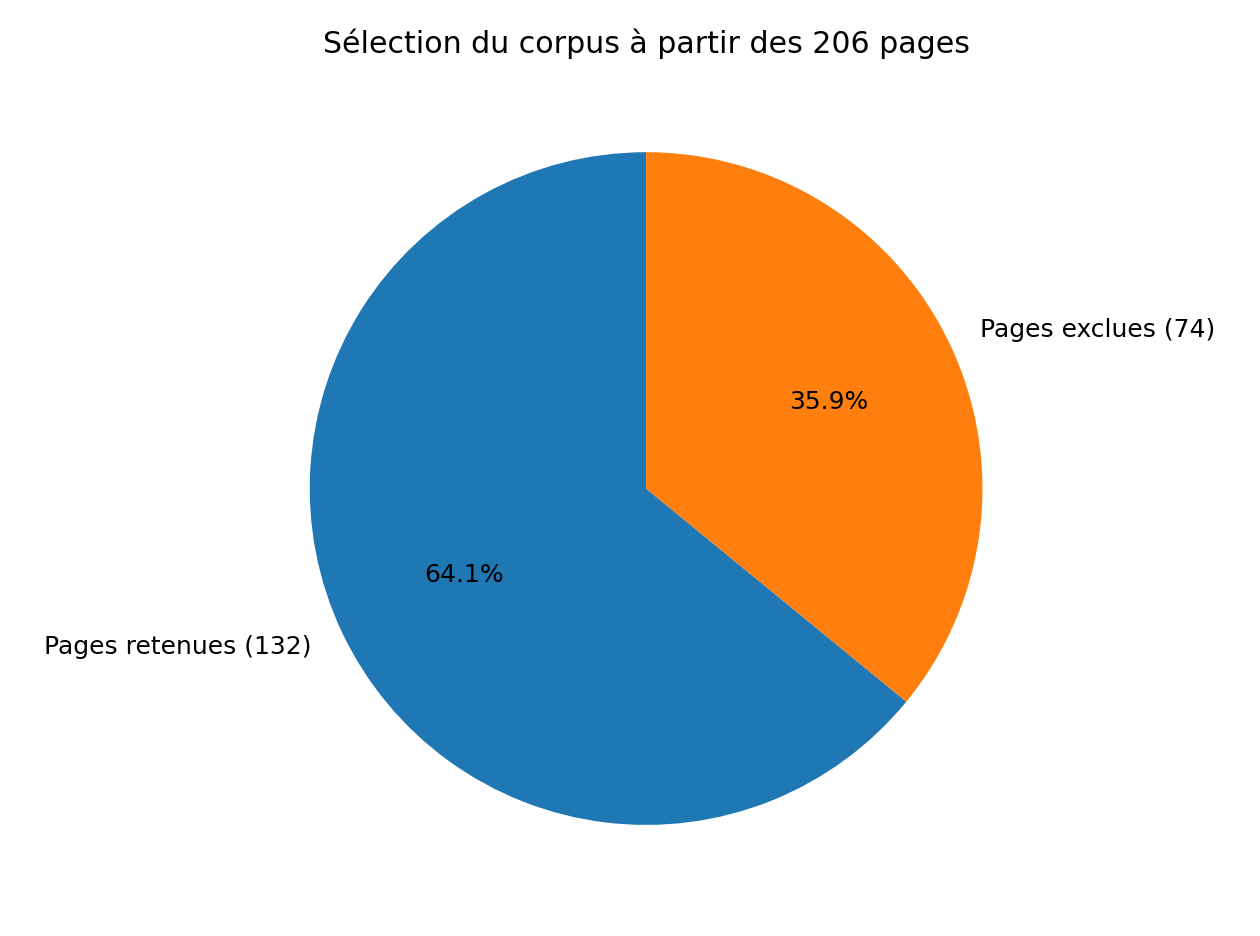
\includegraphics[width=0.64\textwidth]{chart_corpus.png}
\caption{Répartition des pages retenues et exclues}
\end{figure}

Les pages conservées portent des métadonnées : numéro PDF, numéro de la thèse, chapitre, section, langue et statut d'inclusion. Le décalage de pagination est stocké explicitement, car les citations du jury doivent pouvoir être vérifiées dans le fichier PDF réel et dans la pagination imprimée.

\subsection{Extraction des doubles colonnes}
Certaines parties insèrent des articles scientifiques en double colonne. Une extraction naïve peut lire alternativement les lignes des deux colonnes et produire des phrases incohérentes. Le pipeline utilise les blocs PyMuPDF, triés par coordonnées, puis recolle les césures de fin de ligne et normalise les ligatures.

Les tests vérifient également la conservation des nombres scientifiques. Une première règle trop agressive supprimait des valeurs légitimes ; elle a été corrigée pour ne retirer que les numéros isolés identifiés comme pieds de page.

\subsection{Corpus, acronymes et jeu d'évaluation}
Vingt-cinq acronymes sont extraits de la page officielle des acronymes. Ils servent de gazetteer pour reconnaître les entités dans les questions. Le jeu d'évaluation contient 24 questions françaises : six sémantiques, six relationnelles, six hybrides et six hors contexte. Seize questions sont utilisées pour l'entraînement et huit pour le test.

La vérité terrain est définie à la granularité de la page. Un chunk est pertinent si sa page appartient aux pages de référence de la question. Ce choix rend les méthodes comparables malgré des frontières de chunks différentes.

\section{Méthodes de chunking}
\subsection{Fixed-size}
La segmentation fixe découpe le texte selon une taille cible. Elle est simple et rapide, mais elle peut couper une phrase ou séparer une définition de son explication. Un overlap réduit cette perte au prix d'une redondance plus élevée.

\subsection{Sentence-based}
Cette méthode regroupe des phrases complètes. Elle respecte la syntaxe mais peut créer des chunks très courts lorsque le texte contient des titres ou des listes. Elle dépend également de la qualité de la segmentation en phrases dans les passages scientifiques.

\subsection{Paragraph-based}
La méthode par paragraphes conserve les unités discursives naturelles. Dans la thèse, les définitions et les résultats sont souvent exprimés dans un paragraphe cohérent, ce qui explique les bonnes performances mesurées. Elle produit 680 chunks dans la configuration finale.

\subsection{Sliding-window}
Une fenêtre glissante conserve un chevauchement entre chunks successifs. Elle améliore la continuité du contexte, mais augmente le nombre de passages proches et peut réduire la diversité des top résultats.

\subsection{Recursive splitting}
Le découpage récursif tente successivement les séparateurs les plus structurants : section, paragraphe, phrase puis caractères. Il constitue une solution robuste lorsque la structure du texte varie.

\subsection{Semantic chunking}
Le chunking sémantique compare les embeddings de phrases successives et crée une frontière lorsque la similarité chute. Il cherche à détecter un changement de thème, mais son résultat dépend du modèle de référence et du seuil.

\subsection{Document-structure}
Cette méthode suit les titres de chapitre, section et sous-section. Elle conserve la structure du manuscrit, mais peut produire des passages de tailles très différentes. Des règles de sous-segmentation sont nécessaires pour les sections longues.

\subsection{Métriques de comparaison}
Pour chaque méthode, le pipeline calcule le nombre de chunks, les longueurs, le temps, la similarité intra, la similarité inter, Precision@5, Recall@5 et F1@5. La similarité intra mesure la cohérence entre les phrases d'un même chunk. La similarité inter mesure la redondance moyenne entre centroïdes de chunks.

\begin{equation}
F1@k = 2 \times \frac{Precision@k \times Recall@k}{Precision@k + Recall@k}
\end{equation}

\section{Représentations vectorielles}
\subsection{TF-IDF mot et caractères}
TF-IDF mot représente l'importance des termes. La variante par n-grammes de caractères résiste mieux aux variations morphologiques et aux acronymes. Ces représentations sont rapides et interprétables, mais peu adaptées aux reformulations cross-lingues.

\subsection{HashingVectorizer}
Le hashing transforme les tokens en dimensions fixes sans stocker un vocabulaire. Il est rapide et léger, mais les collisions peuvent réduire la précision et les dimensions ne possèdent pas une interprétation directe.

\subsection{SVD 128 et SVD 256}
La réduction SVD applique une projection latente aux matrices TF-IDF. Elle rapproche certains textes selon leurs cooccurrences et réduit la mémoire, mais ne suffit pas à résoudre la différence entre français et anglais.

\subsection{Multilingual MiniLM}
Le modèle \tech{paraphrase-multilingual-MiniLM-L12-v2} produit des vecteurs de 384 dimensions. Il est exécuté localement. Son rôle n'est pas de générer du texte, mais de transformer le sens des phrases en nombres. La question française « vague de froid » devient ainsi proche d'un passage anglais contenant \textit{cold wave}.

\subsection{Représentation hybride}
La représentation hybride concatène ou fusionne une composante TF-IDF avec MiniLM. Elle combine les mots exacts et le sens, au prix d'une dimension et d'un temps d'encodage supérieurs. Dans les mesures finales, MiniLM seul obtient le meilleur classement global.

\section{Vector Store et retrieval}
\subsection{FAISS IndexFlatIP}
Les embeddings sont normalisés L2, puis insérés dans \tech{IndexFlatIP}. Le produit scalaire équivaut alors à la similarité cosinus. L'index est exact : avec 680 chunks, il n'est pas nécessaire d'utiliser une approximation susceptible de perdre des résultats.

\subsection{BM25 et fusion RRF}
BM25 complète FAISS en privilégiant les termes exacts. La fusion RRF donne un score selon le rang :
\begin{equation}
RRF(d) = \sum_{r \in R} \frac{1}{k + rank_r(d)}
\end{equation}
avec $R$ l'ensemble des classements et $k$ une constante de stabilisation.

Les scores FAISS, BM25 et RRF ne doivent pas être comparés directement. Un score BM25 normalisé à 1,000 ne signifie pas qu'il est supérieur à une similarité FAISS de 0,776. L'analyse porte sur la pertinence des passages et sur les métriques de classement.

\subsection{Projection PCA}
La PCA réduit les 384 dimensions à deux composantes pour l'affichage. Chaque point représente un chunk. Les huit groupes visibles indiquent des zones sémantiques, sans constituer une preuve scientifique de huit thèmes stricts. La projection est un outil de diagnostic et de présentation.

\section{Construction du Knowledge Graph}
\subsection{Entités et normalisation}
Le gazetteer issu des acronymes est complété par des entités du corpus et du jeu d'évaluation. Les alias sont normalisés : \textit{WMO} et \textit{World Meteorological Organization} désignent le même nœud. Chaque entité possède un nom, un type, un nombre d'occurrences et des centralités.

\subsection{Relations et provenance}
Les relations sont créées à partir de motifs explicites, d'associations validées et de cooccurrences pondérées. Chaque relation conserve \tech{chunk\_id}, \tech{excerpt}, \tech{confidence} et \tech{extraction\_method}. Cette structure permet de cliquer sur une arête dans Aura et de retrouver le passage source.

\subsection{NetworkX, Louvain et Neo4j Aura}
NetworkX constitue la source locale pour calculer la densité, les composantes et les centralités. Louvain détecte les communautés. Neo4j Aura reçoit ensuite les nœuds et relations par des opérations \tech{MERGE} idempotentes. Une seconde synchronisation conserve donc les mêmes totaux.

\section{Q-Learning et orchestration LangGraph}
\subsection{États et actions}
L'espace comprend 16 états obtenus par le produit de trois caractéristiques : type de question, présence d'une entité graphe et couverture lexicale. Les quatre actions sont \tech{use\_vector}, \tech{use\_graph}, \tech{use\_hybrid} et \tech{abstain}.

\begin{equation}
Q(s,a) \leftarrow Q(s,a) + \alpha \left[r + \gamma \max_{a'}Q(s',a') - Q(s,a)\right]
\end{equation}

Les hyperparamètres sont $\alpha=0{,}1$, $\gamma=0{,}9$ et un epsilon décroissant de 0,30 à 0,05 pendant l'entraînement. En démonstration, la politique est généralement greedy pour garantir un résultat reproductible.

\subsection{Reward et abstention}
Le reward récompense une route conforme au type annoté, un contexte pertinent et une abstention correcte. Une réponse hors contexte est pénalisée. Cette fonction apprend à ne pas utiliser systématiquement la route hybride, plus coûteuse et pas toujours nécessaire.

\subsection{Workflow LangGraph}
Le workflow contient cinq étapes visibles dans l'interface : \tech{feature\_extraction}, \tech{q\_learning\_policy}, \tech{execute\_route}, \tech{context\_verification} et \tech{answer\_and\_reward}. L'état est transmis d'un nœud au suivant et enrichi avec la route, les chunks, le sous-graphe et le score de contexte.

\section{Architecture globale du système}

L'architecture sépare volontairement une phase hors ligne, coûteuse mais exécutée une seule fois, et une phase en ligne optimisée pour la démonstration. La phase hors ligne prépare le corpus, compare les méthodes, entraîne la politique et sérialise les artefacts. La phase en ligne charge ces artefacts en mémoire, analyse la requête et exécute uniquement la route sélectionnée.

Cette séparation garantit la reproductibilité des métriques et évite de recalculer les sept méthodes de segmentation ou les sept représentations à chaque question. La Figure~\ref{fig:architecture-globale} synthétise les flux de données entre le document source, FAISS, NetworkX, Neo4j Aura, le moteur agentique, l'API FastAPI et l'interface React.

\begin{landscape}
\begin{figure}[H]
\centering
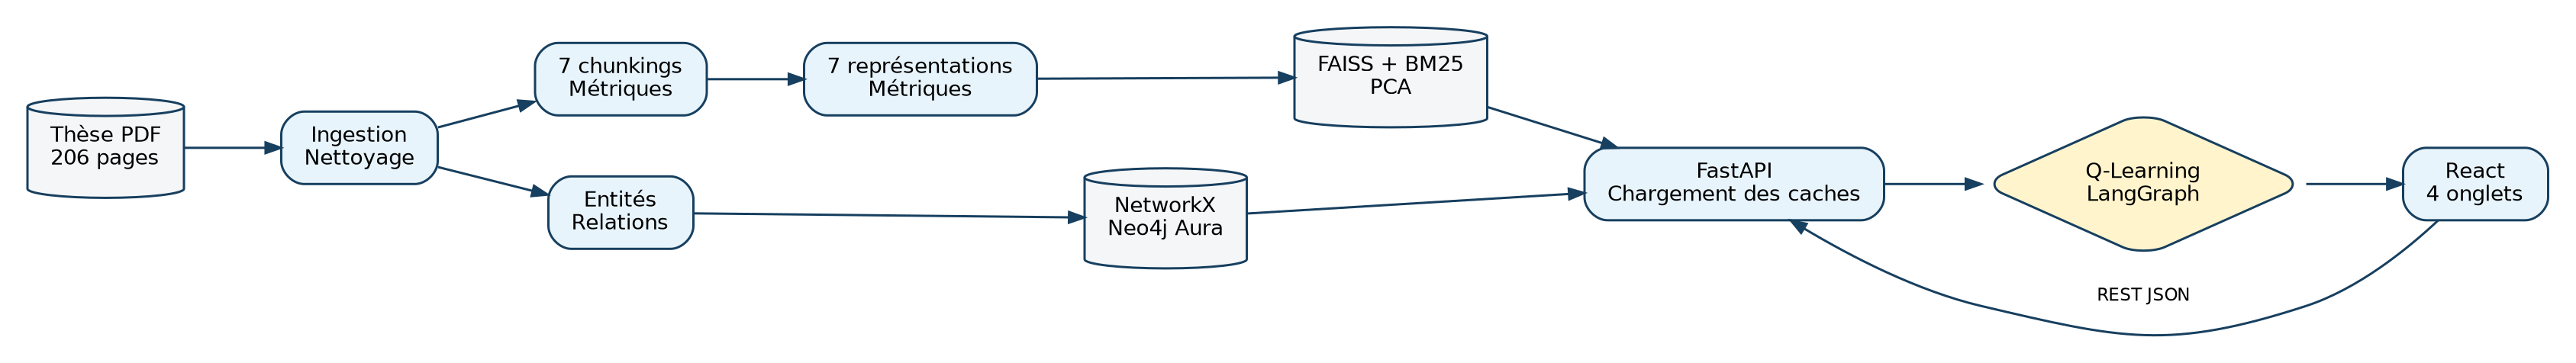
\includegraphics[width=0.96\linewidth]{uml_architecture.png}
\caption{Architecture générale hors ligne et en ligne}
\label{fig:architecture-globale}
\end{figure}
\end{landscape}

\section{Modélisation UML du système}
\subsection{Diagramme de cas d'utilisation global}
Le principal acteur est l'utilisateur qui interroge le corpus et explore les preuves. L'administrateur technique construit les artefacts et vérifie la connexion Aura. Les cas d'utilisation mettent en évidence que la consultation d'une réponse inclut le routage et la récupération du contexte.

\begin{figure}[H]
\centering
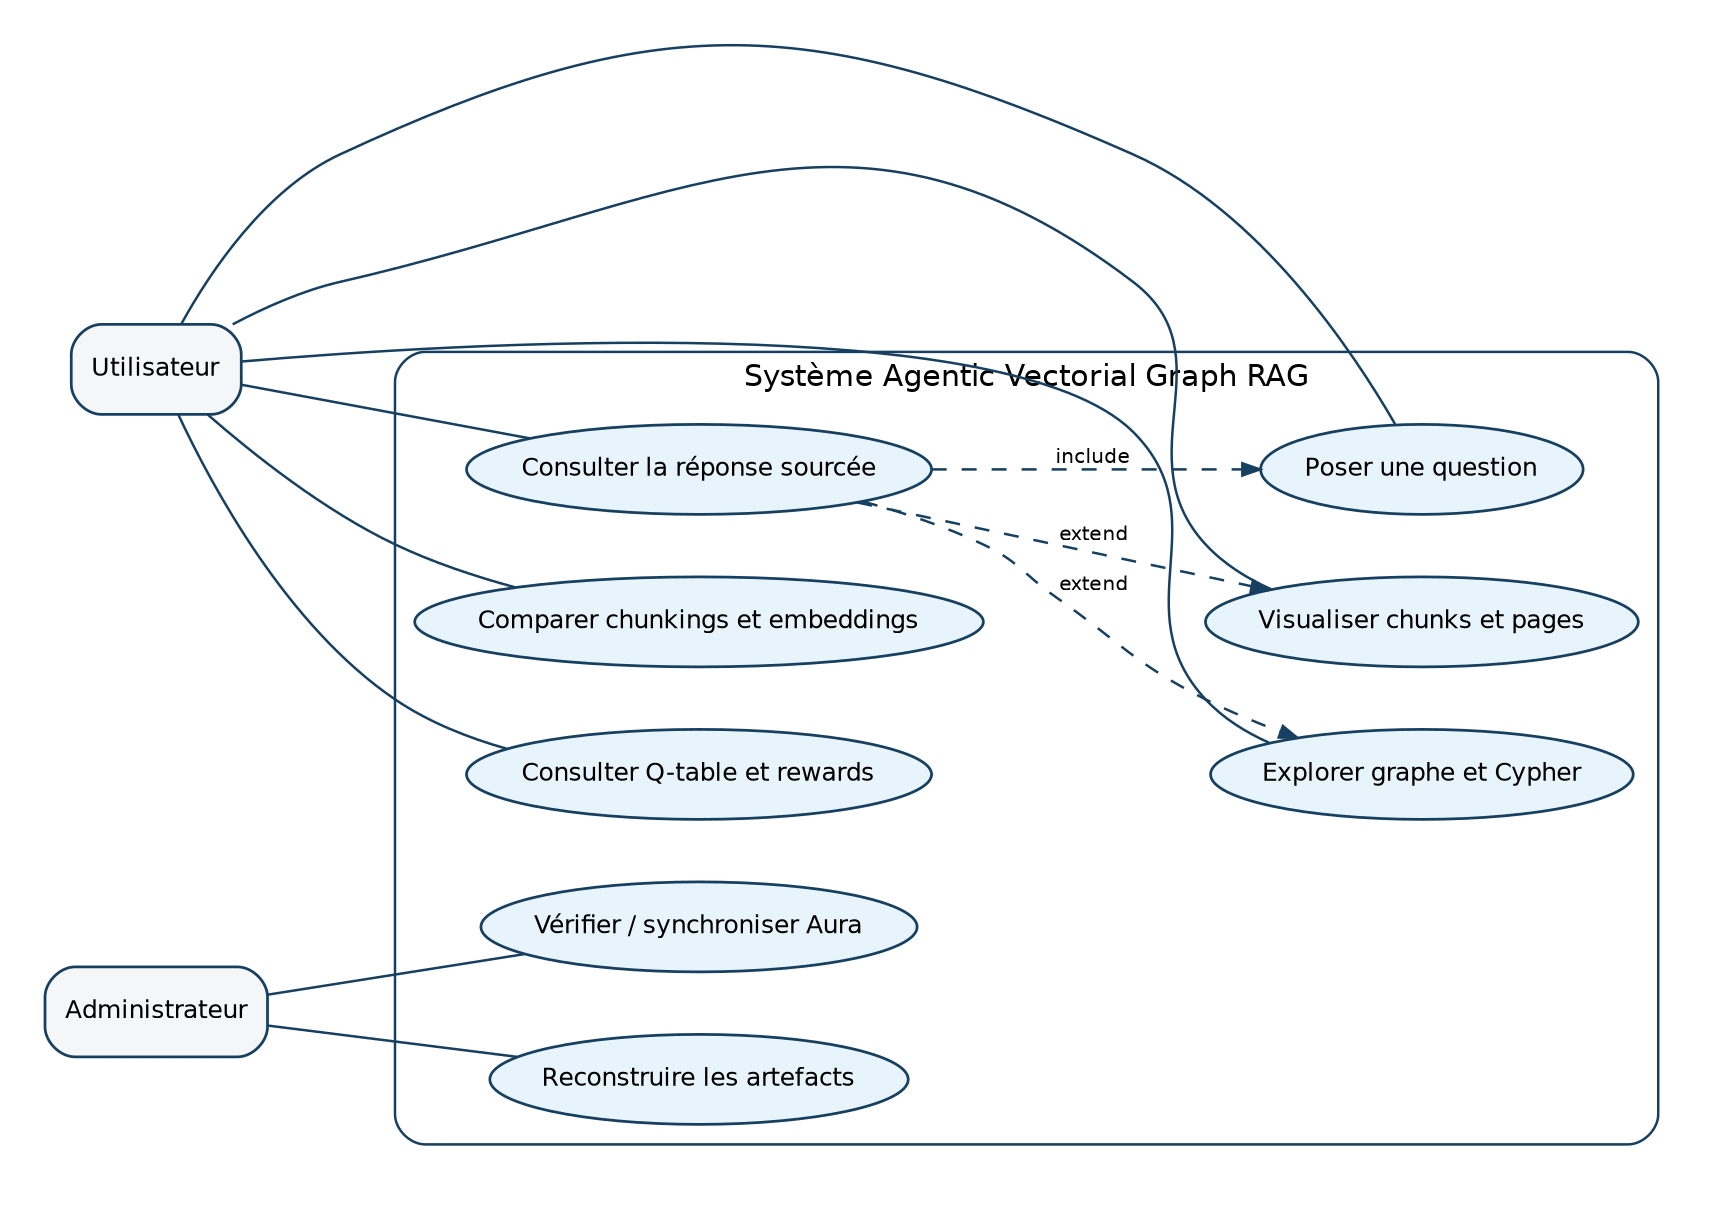
\includegraphics[width=0.94\textwidth]{uml_usecase.png}
\caption{Diagramme de cas d'utilisation global}
\label{fig:usecase}
\end{figure}

\subsection{Diagramme d'activité du traitement d'une question}
\begin{figure}[H]
\centering
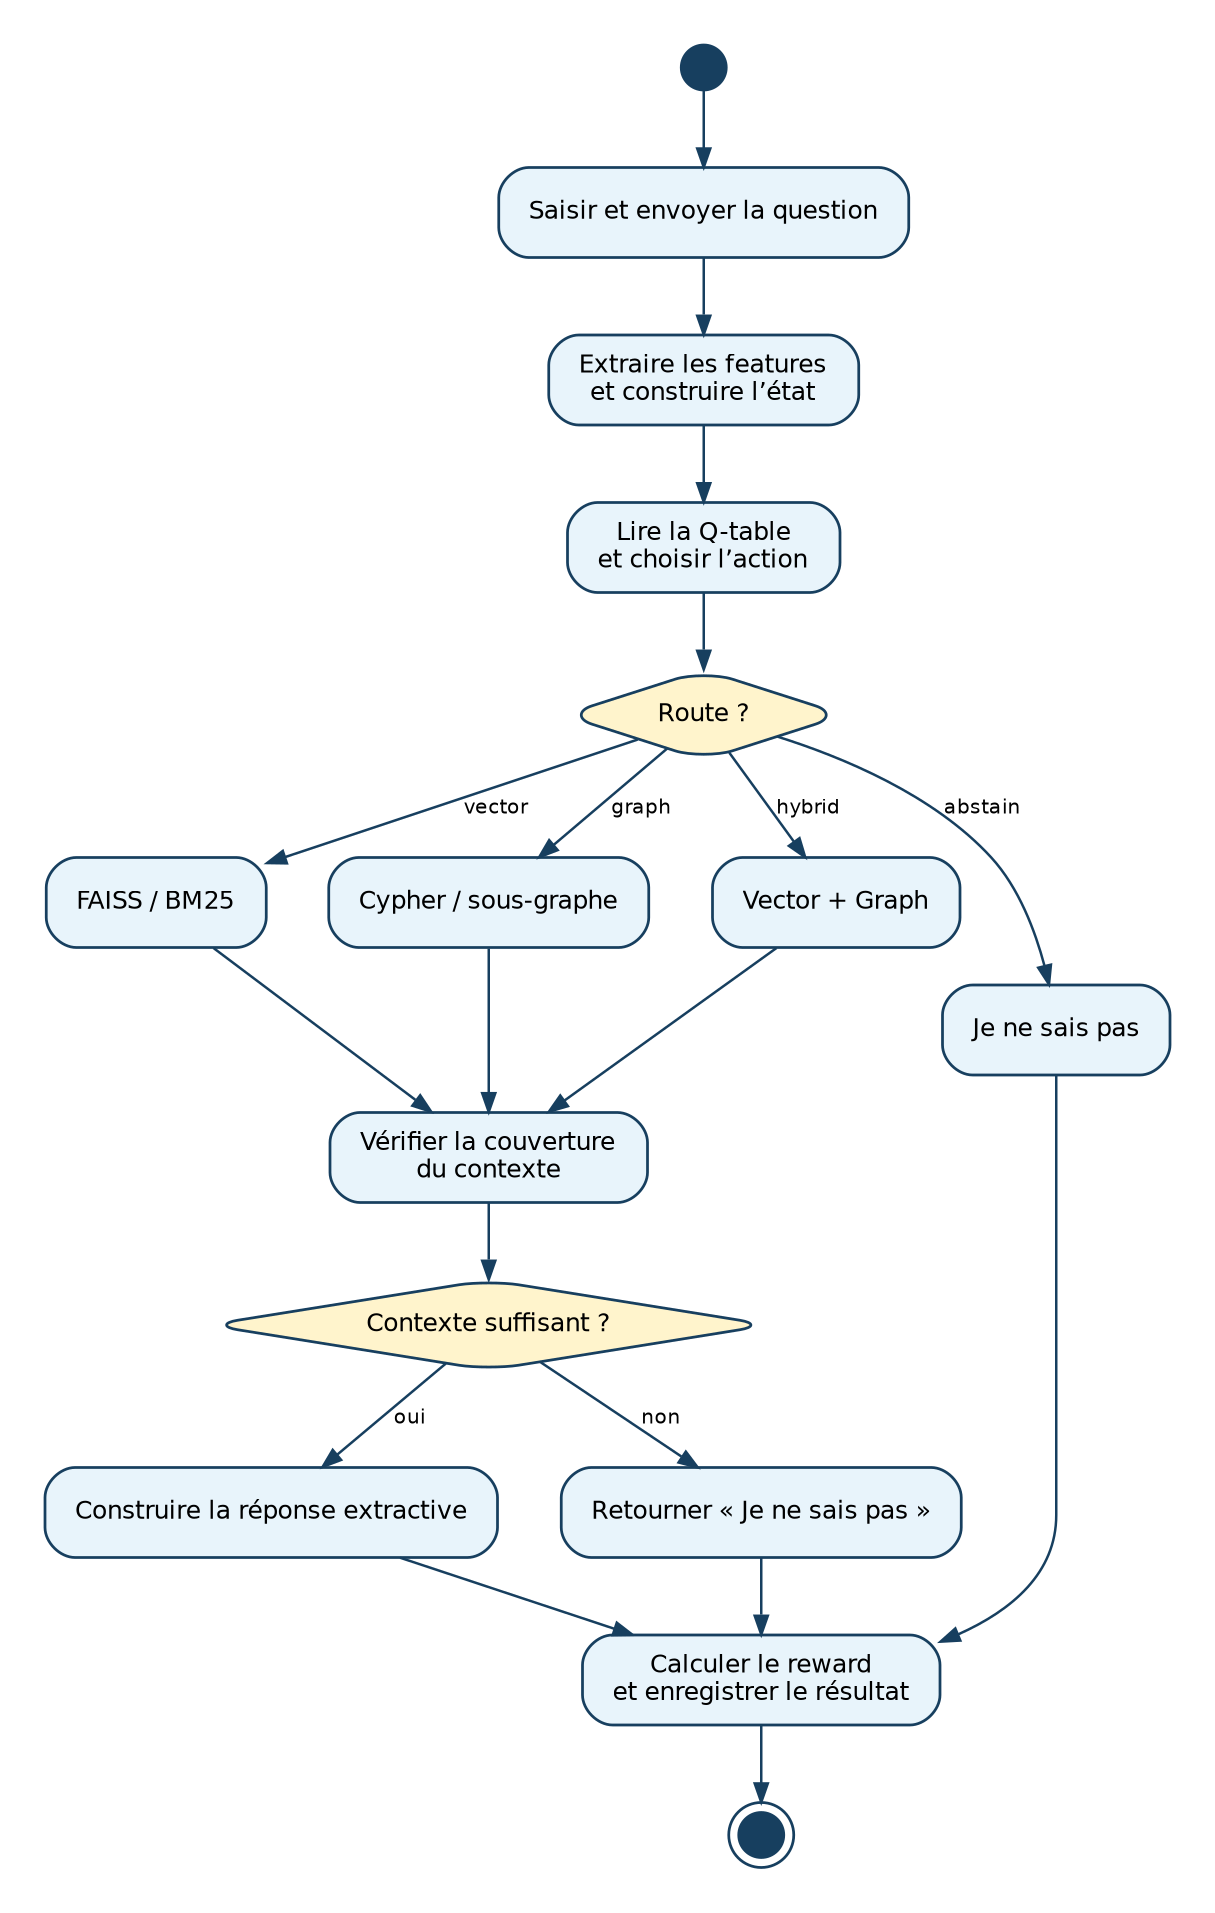
\includegraphics[height=0.67\textheight,keepaspectratio]{uml_activity.png}
\caption{Diagramme d'activité du pipeline agentique}
\label{fig:activity}
\end{figure}

\subsection{Diagramme de séquence d'une requête hybride}
\begin{landscape}
\begin{figure}[H]
\centering
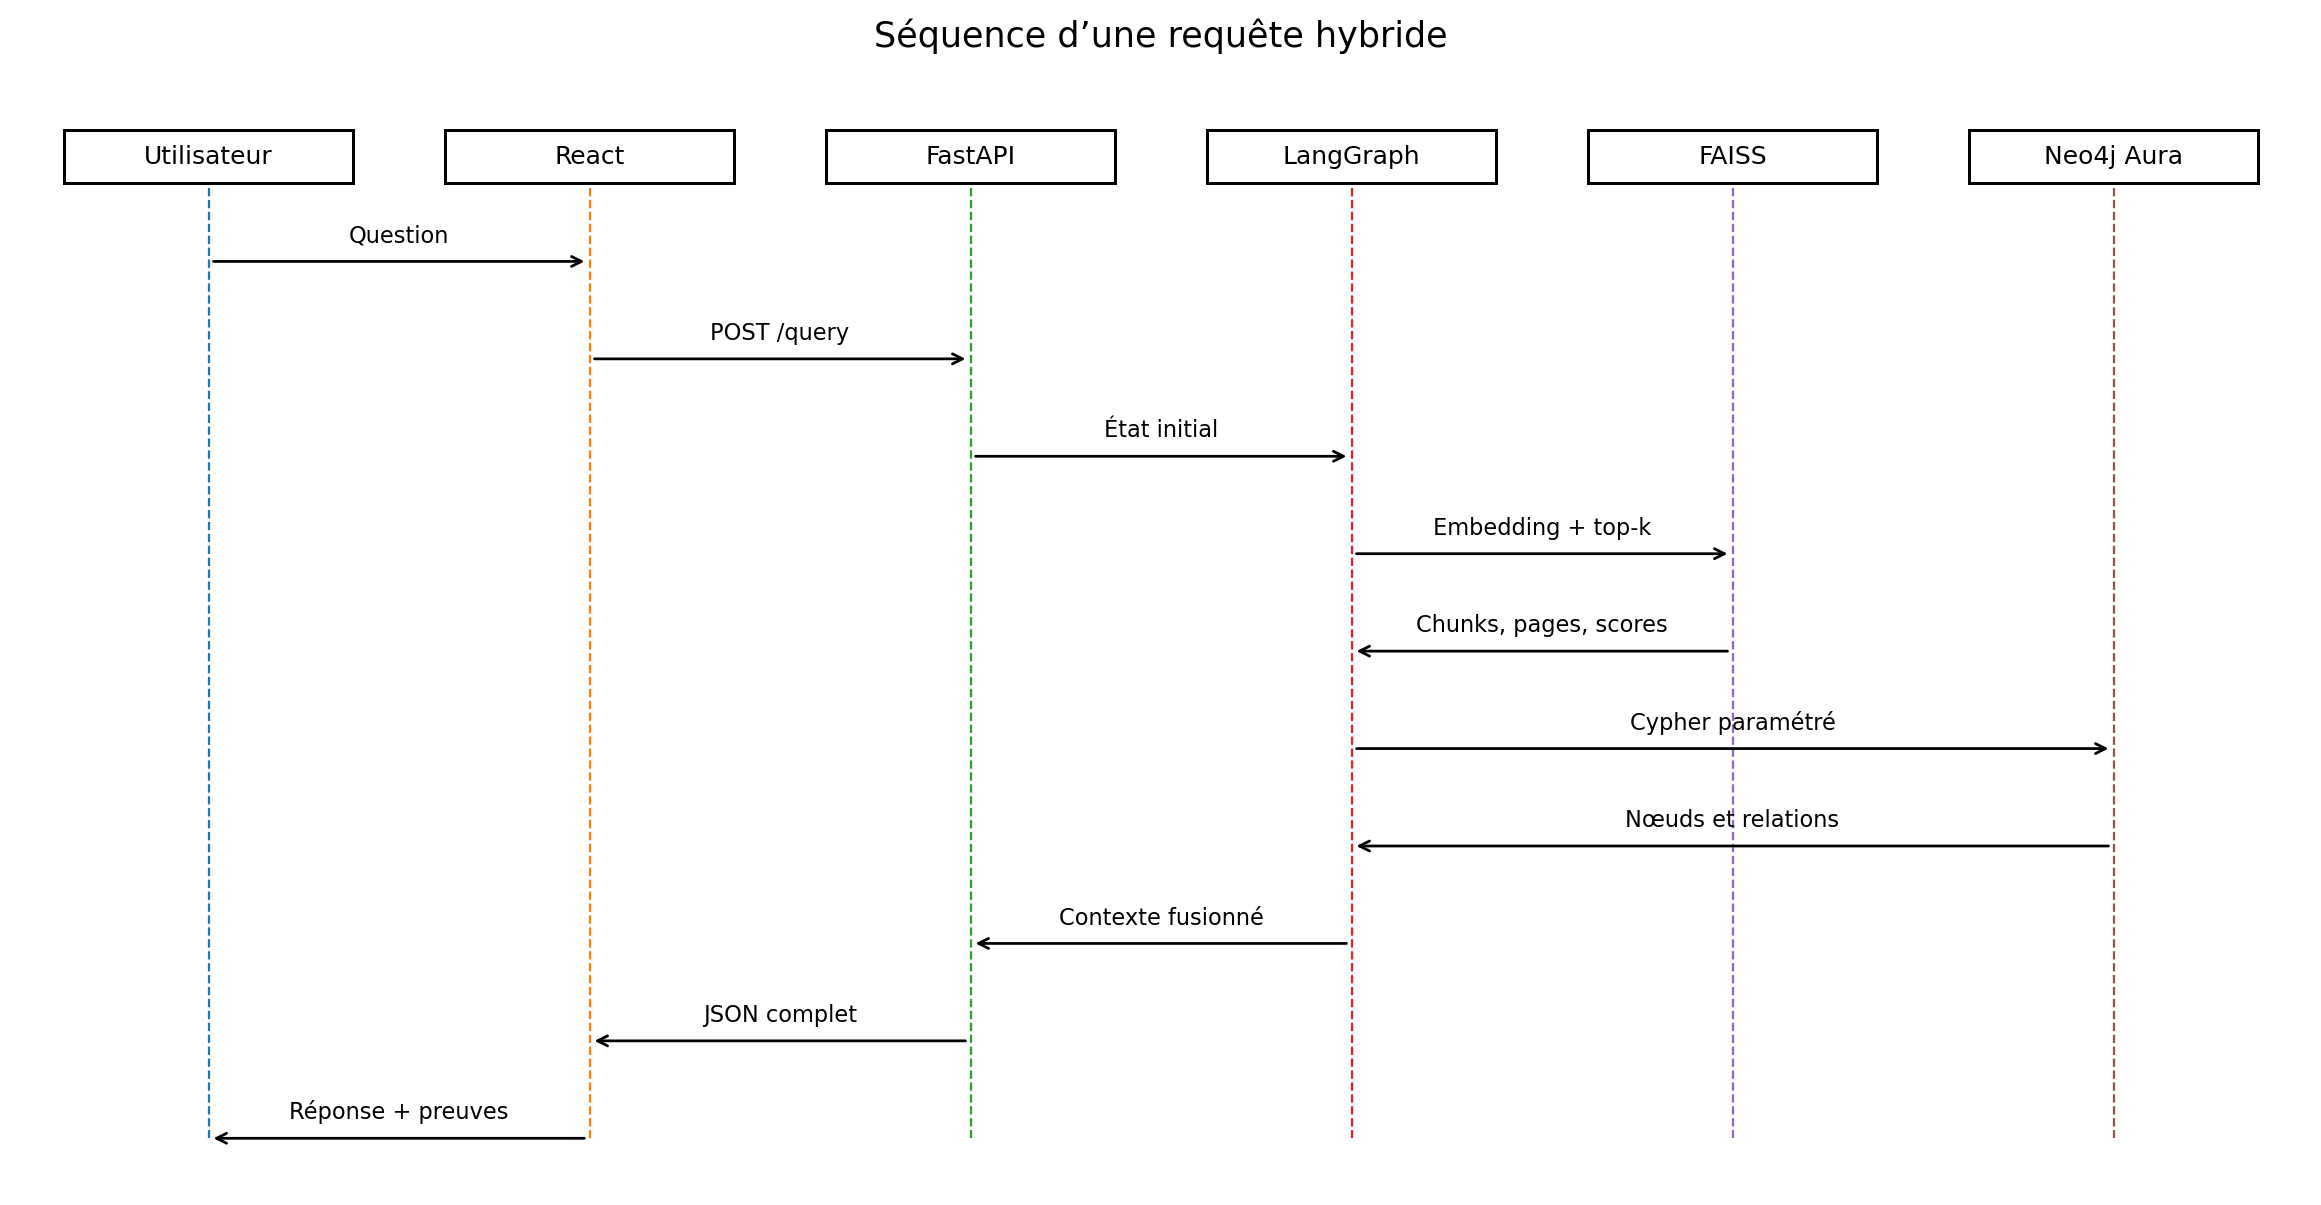
\includegraphics[width=0.94\linewidth]{uml_sequence.png}
\caption{Diagramme de séquence d'une requête hybride}
\label{fig:sequence}
\end{figure}
\end{landscape}

\subsection{Diagramme de composants}
\begin{figure}[H]
\centering
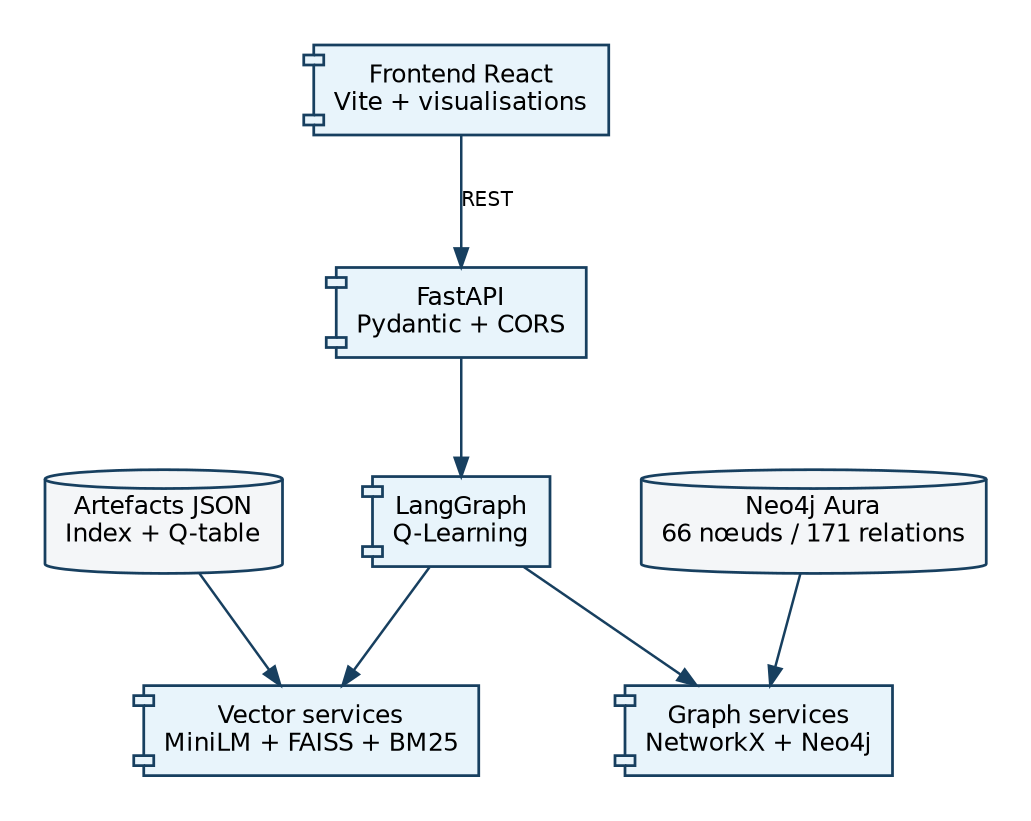
\includegraphics[width=0.78\textwidth]{uml_components.png}
\caption{Diagramme de composants du prototype}
\label{fig:components}
\end{figure}

\subsection{Diagramme de déploiement}
\begin{landscape}
\begin{figure}[H]
\centering
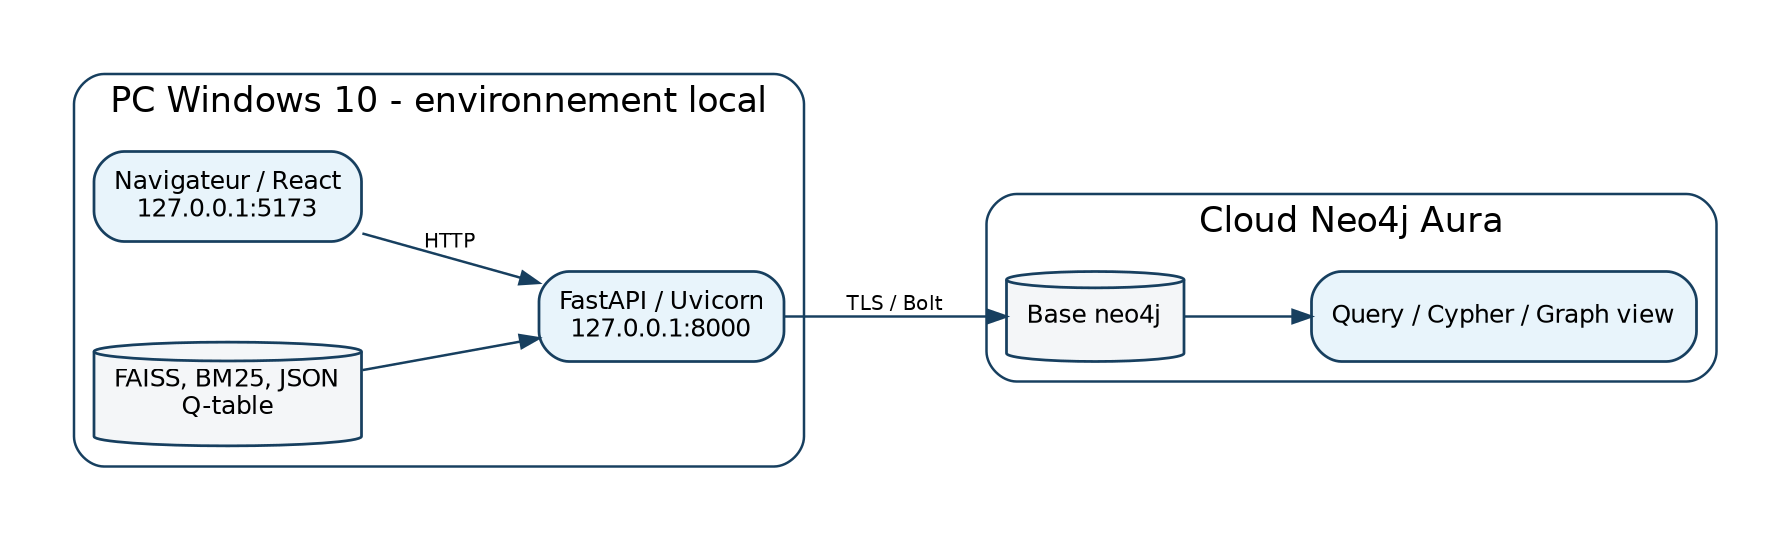
\includegraphics[width=0.92\linewidth]{uml_deployment.png}
\caption{Diagramme de déploiement local et cloud}
\label{fig:deployment}
\end{figure}
\end{landscape}

\section{Architecture de l'API et de l'interface}
Les quatre routes canoniques sont \tech{POST /query}, \tech{GET /vectorial}, \tech{GET /graph} et \tech{GET /agentic}. Elles sont complétées par des sous-routes pour les tableaux, la PCA, les communautés et les sous-graphes. Swagger est disponible sur \tech{/docs}.

L'interface React possède quatre onglets : Query, Vectorial RAG, Graph RAG et Agentic RAG. Le frontend ne recalcule aucune métrique ; il lit les valeurs produites par le backend. Cette séparation garantit que les chiffres affichés correspondent aux artefacts expérimentaux.

\section{Protocole d'évaluation}
La comparaison du chunking utilise un modèle d'embedding de référence constant. Ensuite, les sept représentations sont comparées sur le chunking gagnant. Cette méthode évite 49 combinaisons et conserve une comparaison équitable.

Les métriques de ranking sont calculées sur les pages de référence : Precision@5, Recall@5, F1@5, MAP, MRR et NDCG@5. Les questions hors contexte évaluent l'abstention. Le test final contient deux questions de chaque type.


\section{Définition détaillée des métriques}
\subsection{Precision, Recall et F1 à k}
Pour une question $q$, les documents pertinents sont les chunks dont la page appartient à la vérité terrain. Si $Rel_q$ est l'ensemble pertinent et $Top_k(q)$ le classement retourné :
\begin{align}
Precision@k(q) &= \frac{|Top_k(q) \cap Rel_q|}{k} \\
Recall@k(q) &= \frac{|Top_k(q) \cap Rel_q|}{|Rel_q|}
\end{align}

Ces deux valeurs répondent à des questions différentes. La précision indique la proportion de résultats utiles dans les cinq premiers. Le rappel indique la part des pages attendues effectivement retrouvée. Le F1 équilibre les deux.

\subsection{MAP et MRR}
L'Average Precision additionne la précision aux rangs où apparaît un élément pertinent. MAP est la moyenne sur les questions. MRR se concentre sur le premier résultat pertinent :
\begin{equation}
MRR = \frac{1}{|Q|}\sum_{q \in Q}\frac{1}{rank_q}
\end{equation}

Une valeur MRR élevée signifie qu'un utilisateur rencontre rapidement une source utile. Cette métrique est particulièrement adaptée à l'interface, qui affiche seulement quelques chunks en priorité.

\subsection{NDCG}
NDCG réduit le poids des résultats pertinents placés loin dans le classement. Avec des gains binaires :
\begin{equation}
DCG@k = \sum_{i=1}^{k}\frac{rel_i}{\log_2(i+1)}, \qquad NDCG@k = \frac{DCG@k}{IDCG@k}
\end{equation}

La valeur est comprise entre 0 et 1. Le score de 0,500 obtenu par MiniLM est le meilleur parmi les sept représentations, mais il montre également qu'une marge d'amélioration subsiste.

\subsection{Similarité intra et inter}
Pour un chunk composé de plusieurs phrases, la similarité intra est la moyenne des cosinus entre embeddings de phrases. Une valeur élevée indique que les phrases abordent un sujet cohérent. La similarité inter compare les centroïdes de chunks distincts ; une valeur trop élevée signale une redondance.

\subsection{Métriques du graphe}
La densité compare le nombre d'arêtes au nombre maximal possible. La degree centrality mesure la proportion de voisins directs. La betweenness centrality identifie les nœuds situés sur de nombreux plus courts chemins. La closeness centrality estime la proximité moyenne d'un nœud avec le reste du graphe.

La modularité évalue la séparation des communautés. Une modularité de 0,281 indique une organisation communautaire réelle mais modérée, ce qui est cohérent avec un petit graphe scientifique fortement connecté autour d'un thème commun.

\section{Modèle de données du pipeline}
Les objets échangés entre l'interface, l'API et les moteurs de récupération conservent la question, l'état agentique, les preuves textuelles, les relations du graphe et la provenance. Cette modélisation simplifiée facilite la validation par Pydantic et garantit que chaque réponse reste traçable jusqu'aux pages et chunks d'origine.

\begin{figure}[H]
\centering
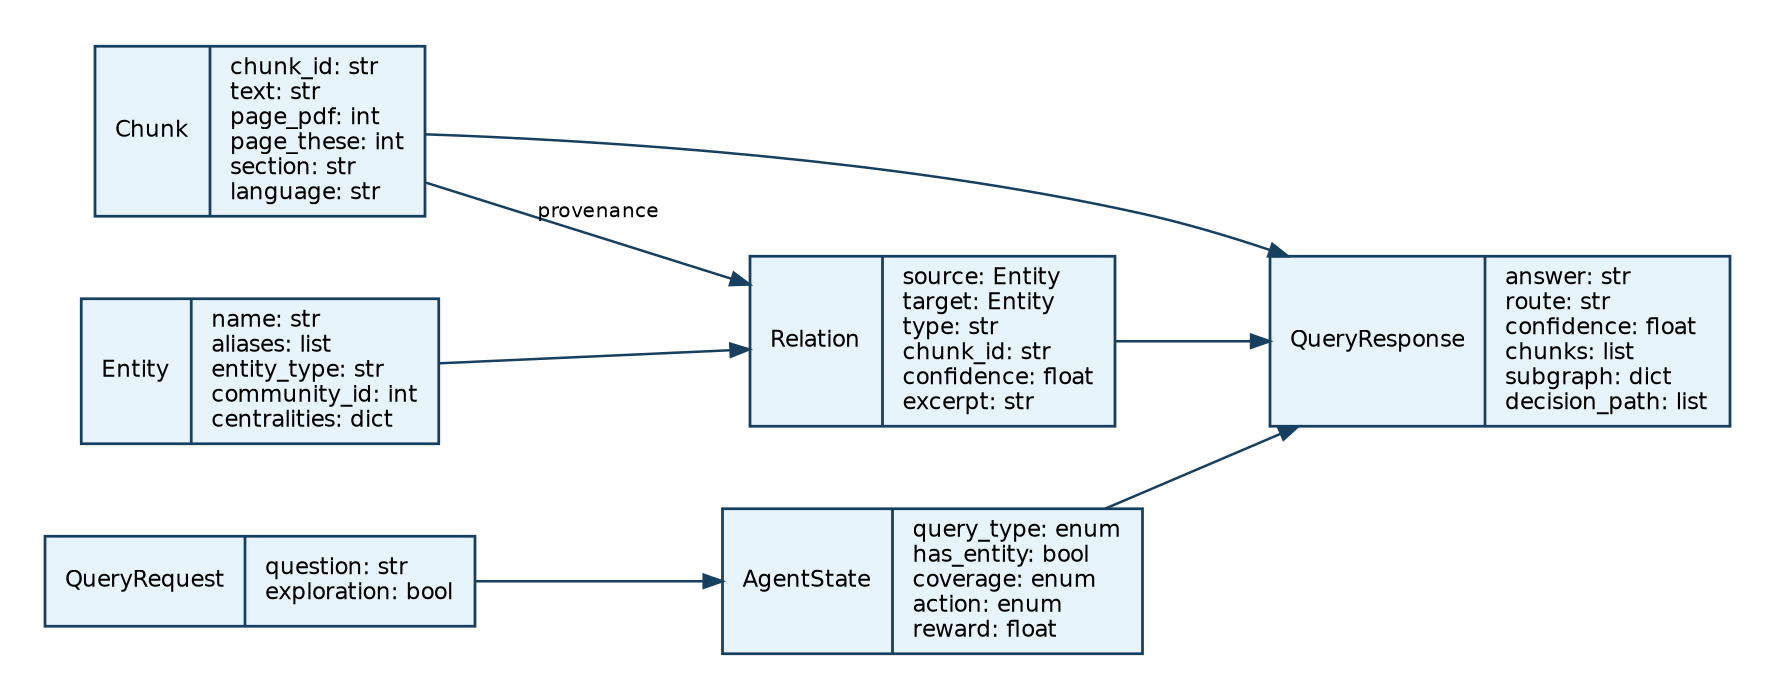
\includegraphics[width=0.98\textwidth]{uml_classes.png}
\caption{Diagramme de classes simplifié des objets échangés}
\label{fig:classes}
\end{figure}

\section{Sécurité, reproductibilité et gestion des secrets}
Les identifiants Aura ne sont jamais inscrits dans les sources ni dans les captures du rapport. Le fichier de configuration local est ignoré par Git. Les réponses de santé n'exposent que l'état de connexion et les totaux. Les requêtes Cypher utilisent des paramètres pour éviter la concaténation directe d'une saisie utilisateur.

La reproductibilité repose sur trois mécanismes : seeds fixes, artefacts persistants et scripts de reconstruction. Chaque tableau de métriques est associé à une exécution. Les tests vérifient qu'une seconde synchronisation Aura ne double pas le nombre de relations.

\section{Conclusion du chapitre}
La conception sépare clairement la phase hors ligne et la phase en ligne. Les étapes coûteuses sont exécutées une fois, tandis que la requête utilisateur exploite des artefacts persistants. Les diagrammes UML montrent que le Q-Learning est intégré au flux de décision et que les sources vectorielle et graphe restent indépendantes mais combinables.

% =============================================================================
% CHAPITRE 3
% =============================================================================
\chapter{Implémentation et Résultats}

\section{Environnements et outils de développement}
Le backend est développé en Python 3.11. Les bibliothèques principales sont PyMuPDF pour l'extraction, scikit-learn pour TF-IDF, SVD et PCA, sentence-transformers pour MiniLM, faiss-cpu pour l'index, NetworkX pour le graphe, le driver Neo4j, LangGraph, FastAPI et pytest. Le frontend utilise React, Vite et des composants de visualisation.

L'environnement Conda \tech{pfa-rag} isole les dépendances. Le modèle MiniLM est téléchargé une fois puis chargé depuis le cache local. Le script \tech{run\_mvp.bat} lance le backend et le frontend, tandis que \tech{rebuild\_artifacts.bat} reconstruit les données expérimentales.

\section{Résultats de l'ingestion}
Le pipeline a extrait les 206 pages sans OCR. Après exclusion des zones non pertinentes, 132 pages, 289 941 caractères et 45 769 mots alimentent le RAG. Sept réparations de frontière de page ont été appliquées et 25 acronymes ont été extraits.

La validation a révélé plusieurs défauts réels au cours du développement : en-têtes de revue conservés, suppression accidentelle de nombres, paragraphes éclatés et césures entre colonnes. Les tests ont permis de corriger ces anomalies avant la comparaison des méthodes.

\begin{table}[H]
\centering
\caption{Bilan réel de l'ingestion}
\begin{tabular}{lr}
\toprule
\textbf{Indicateur} & \textbf{Valeur}\\
\midrule
Pages du PDF & 206\\
Pages retenues & 132\\
Pages exclues & 74\\
Caractères utiles & 289 941\\
Mots utiles & 45 769\\
Acronymes & 25\\
Réparations de frontières & 7\\
OCR nécessaire & Non\\
\bottomrule
\end{tabular}
\end{table}

\section{Comparaison des sept méthodes de chunking}
\begin{table}[H]
\centering
\small
\caption{Résultats réels des méthodes de chunking}
\begin{tabularx}{\textwidth}{lrrrrr}
\toprule
\textbf{Méthode} & \textbf{Chunks} & \textbf{F1@5} & \textbf{Recall@5} & \textbf{Intra} & \textbf{Score global}\\
\midrule
fixed\_size & 416 & 0,266 & 0,528 & 0,417 & 0,622\\
sentence\_based & 413 & 0,234 & 0,472 & 0,394 & 0,302\\
\textbf{paragraph\_based} & \textbf{680} & \textbf{0,282} & \textbf{0,556} & 0,393 & \textbf{0,693}\\
sliding\_window & 478 & 0,278 & 0,528 & 0,384 & 0,573\\
recursive & 504 & 0,237 & 0,500 & \textbf{0,429} & 0,492\\
semantic & 456 & 0,256 & 0,556 & 0,396 & 0,400\\
document\_structure & 299 & 0,234 & \textbf{0,611} & 0,411 & 0,329\\
\bottomrule
\end{tabularx}
\end{table}

\begin{figure}[H]
\centering
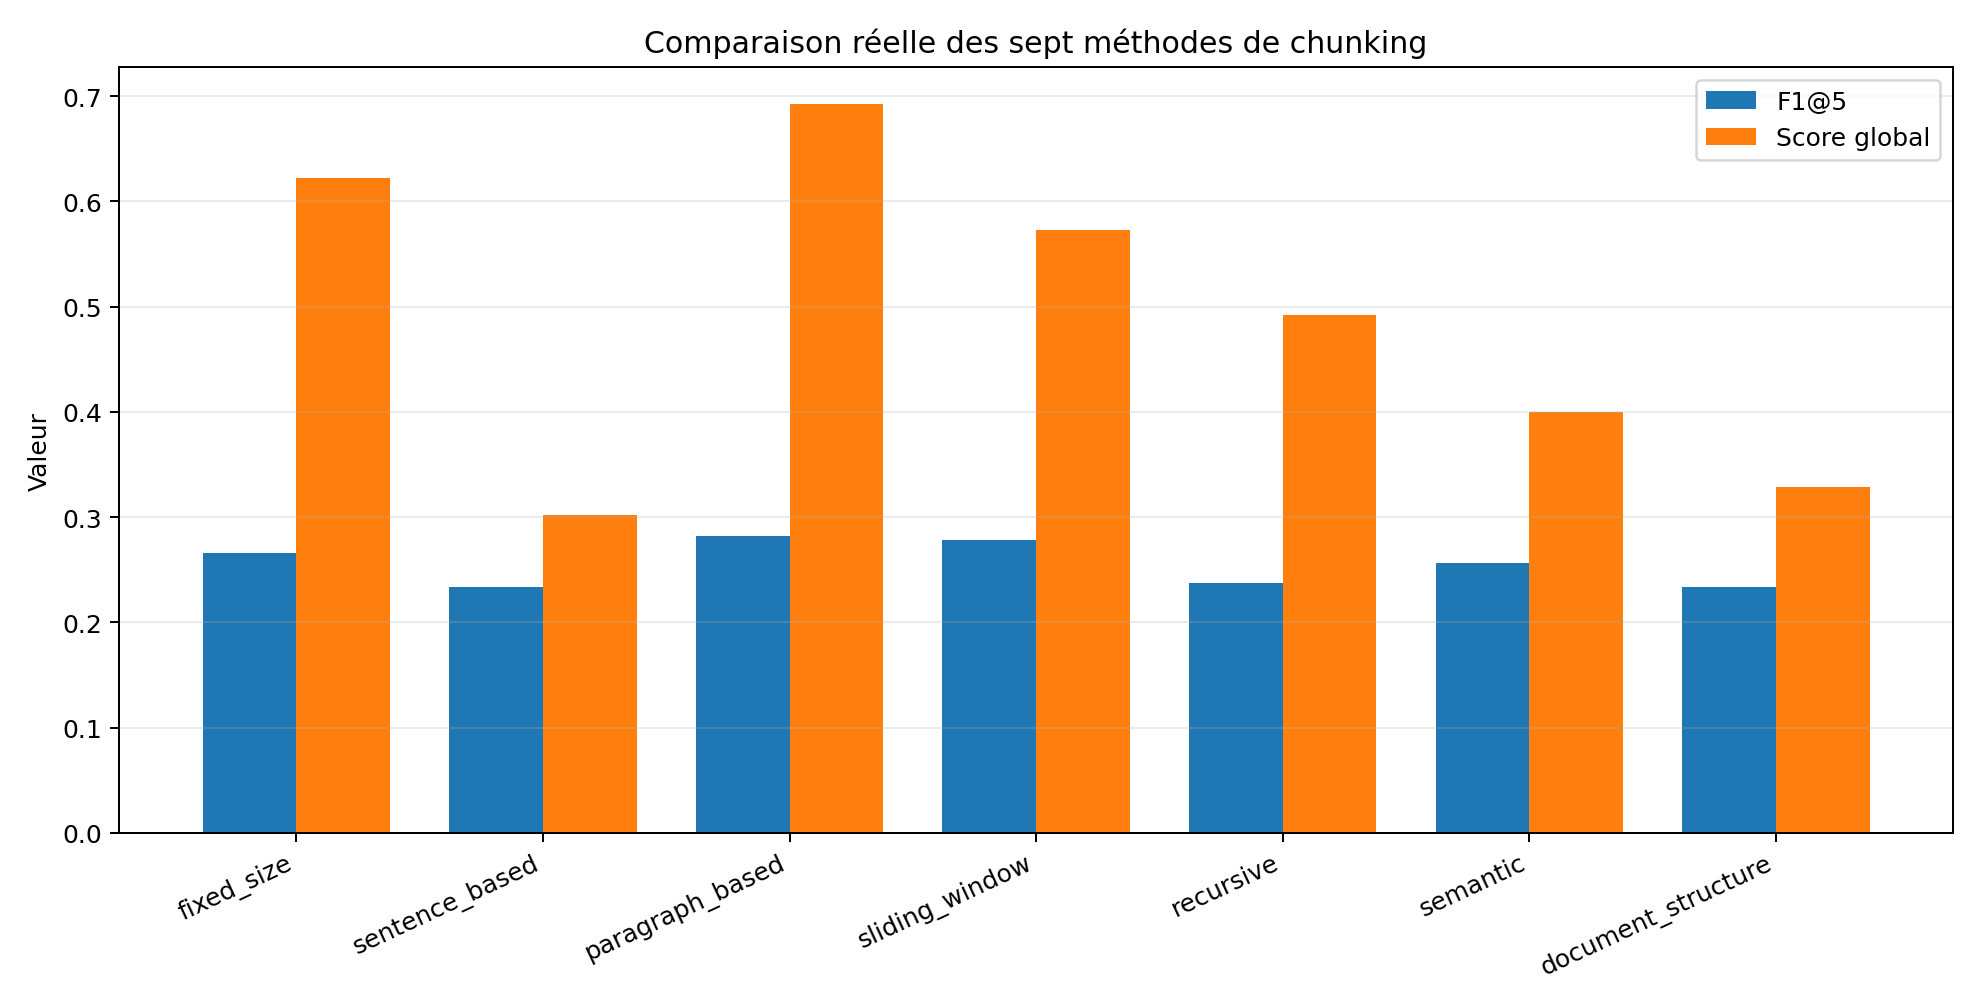
\includegraphics[width=0.96\textwidth]{chart_chunking.png}
\caption{Comparaison de F1@5 et du score global des chunkings}
\end{figure}

La méthode document-structure obtient le Recall@5 le plus élevé, mais son score global est pénalisé par d'autres critères. Paragraph-based atteint le meilleur compromis et devient la méthode de production. Ce résultat est cohérent avec la rédaction scientifique du corpus, organisée en paragraphes argumentatifs.

\section{Comparaison des sept représentations vectorielles}
\begin{table}[H]
\centering
\scriptsize
\caption{Résultats réels des représentations vectorielles}
\begin{tabularx}{\textwidth}{lrrrrrr}
\toprule
\textbf{Représentation} & \textbf{Dim.} & \textbf{F1@5} & \textbf{MAP} & \textbf{MRR} & \textbf{NDCG@5} & \textbf{Temps (s)}\\
\midrule
tfidf\_word & 7 901 & 0,051 & 0,061 & 0,136 & 0,135 & 0,123\\
tfidf\_char\_ngrams & 22 176 & 0,126 & 0,087 & 0,282 & 0,289 & 0,340\\
hashing\_vectorizer & 8 192 & 0,032 & 0,037 & 0,080 & 0,077 & 0,051\\
tfidf\_svd\_128 & 128 & 0,037 & 0,059 & 0,132 & 0,111 & 0,434\\
tfidf\_svd\_256 & 256 & 0,037 & 0,059 & 0,134 & 0,111 & 0,911\\
\textbf{multilingual\_minilm} & \textbf{384} & \textbf{0,282} & \textbf{0,133} & \textbf{0,402} & \textbf{0,500} & 24,208\\
hybrid\_tfidf\_minilm & 512 & 0,159 & 0,118 & 0,282 & 0,327 & 25,587\\
\bottomrule
\end{tabularx}
\end{table}

\begin{figure}[H]
\centering
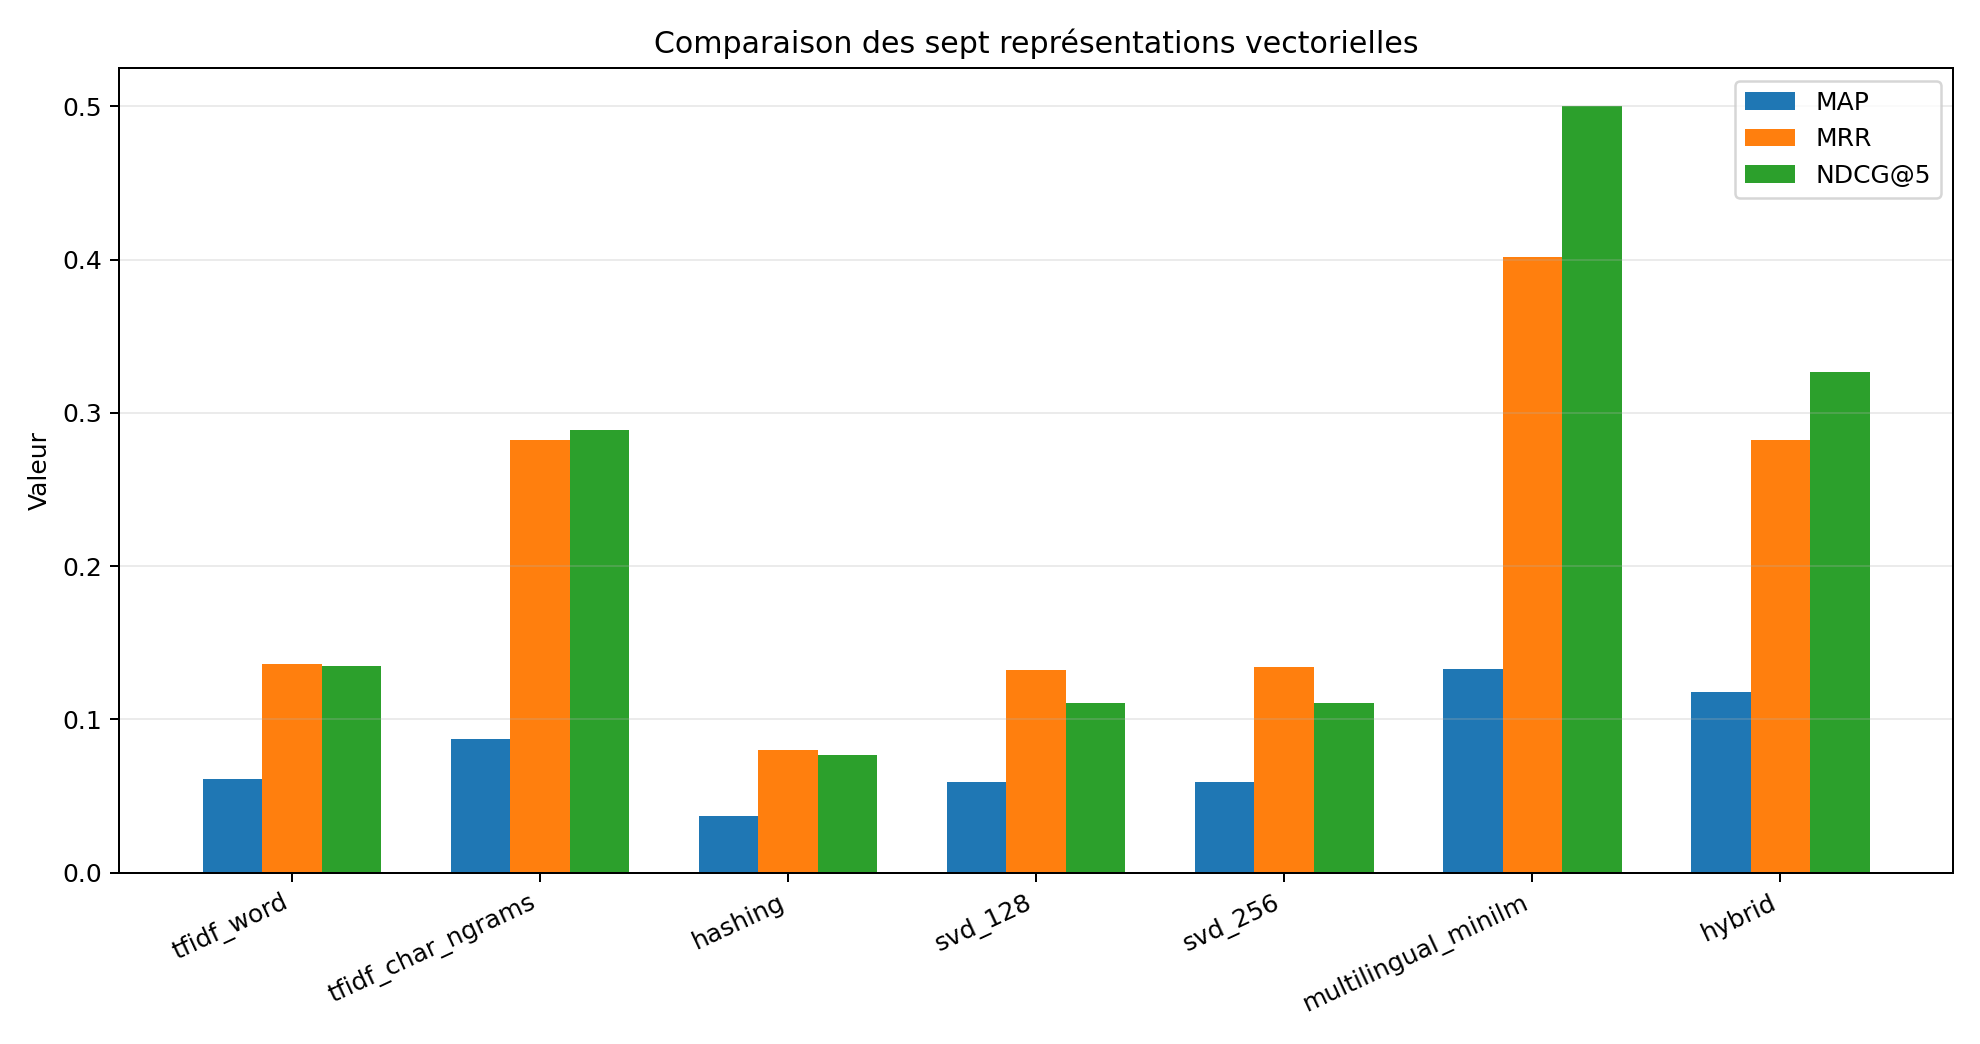
\includegraphics[width=0.96\textwidth]{chart_embeddings.png}
\caption{MAP, MRR et NDCG@5 des représentations vectorielles}
\end{figure}

MiniLM est plus lent à encoder que les méthodes lexicales, mais ce coût n'est payé que lors de la construction. Son avantage sur MRR et NDCG confirme sa capacité à retrouver rapidement un passage pertinent dans un corpus majoritairement anglais à partir d'une question française.

\section{Résultats du Vector RAG}
L'index final contient 680 vecteurs de 384 dimensions. La requête est encodée puis comparée aux chunks. Les résultats affichent l'identifiant, la similarité, la page PDF, la page de la thèse, la section et un extrait.

Pour la question sur le blocage scandinave, FAISS renvoie des passages de pages 23, 22 et 89 avec des similarités 0,776, 0,757 et 0,716. Ces passages décrivent directement l'advection d'air froid depuis l'Arctique ou la Sibérie et l'affaiblissement des vents d'ouest. BM25 classe au contraire des pages générales sur les objectifs de la thèse. Cet exemple illustre l'intérêt du retrieval sémantique.

\begin{landscape}
\begin{figure}[H]
\centering
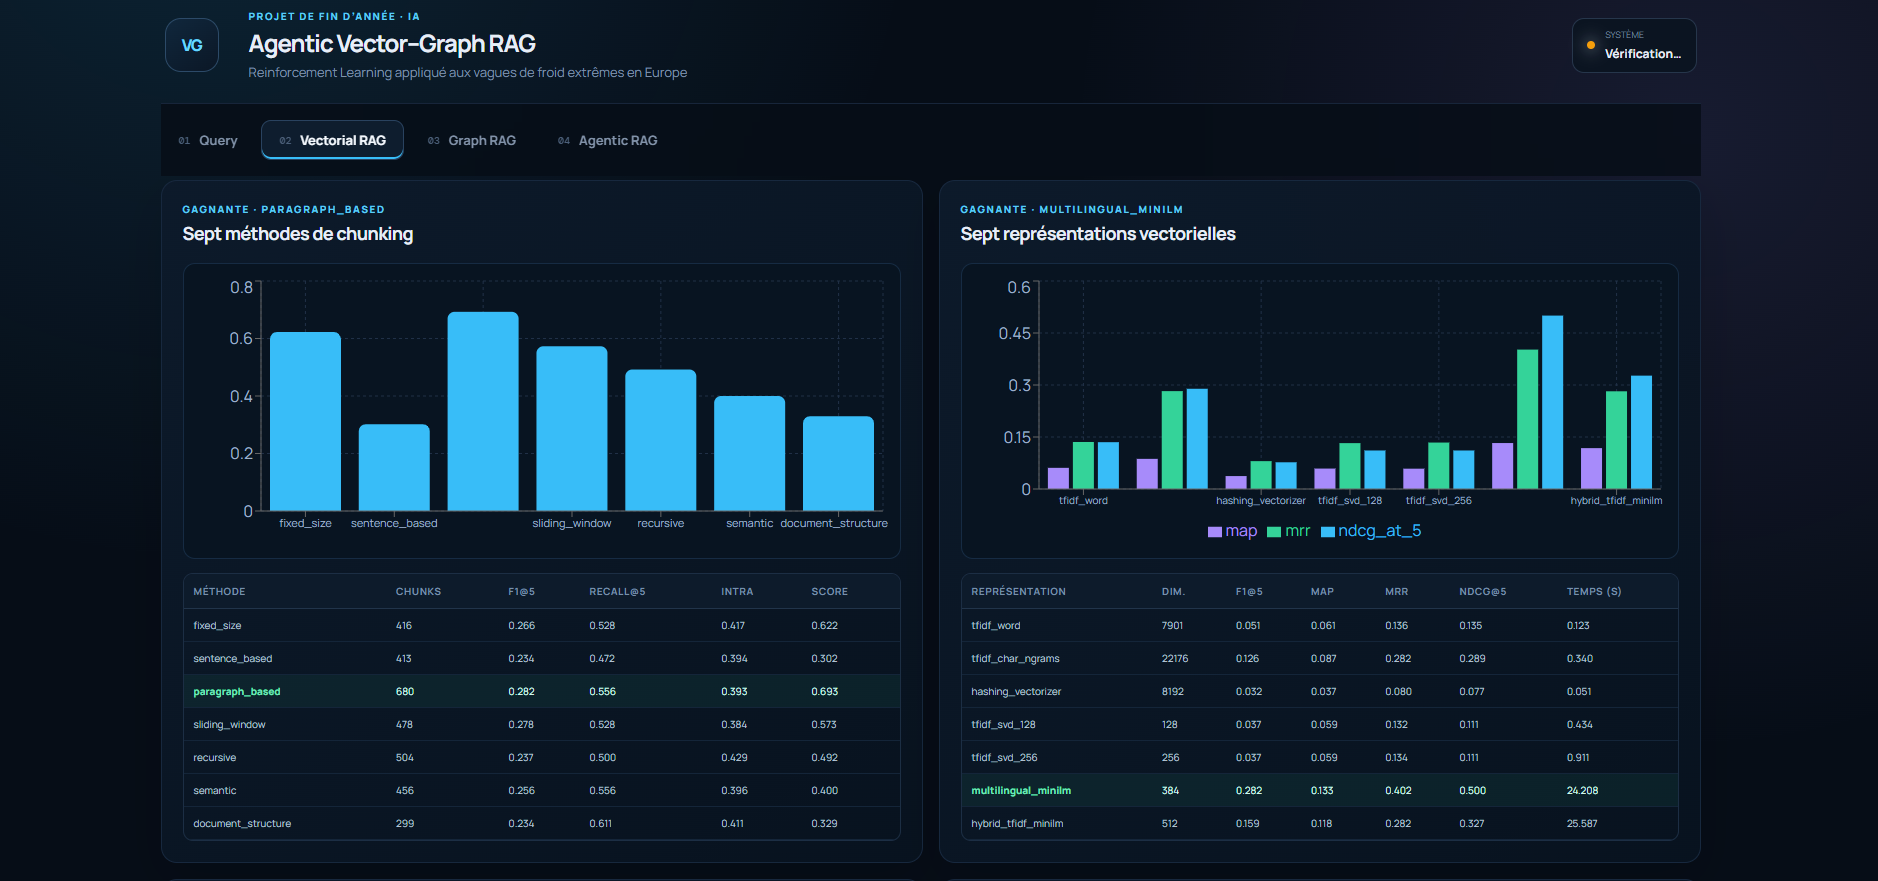
\includegraphics[width=0.95\linewidth]{interface_vector_metrics.png}
\caption{Onglet Vectorial RAG : comparaison des chunkings et embeddings}
\end{figure}
\end{landscape}

\begin{landscape}
\begin{figure}[H]
\centering
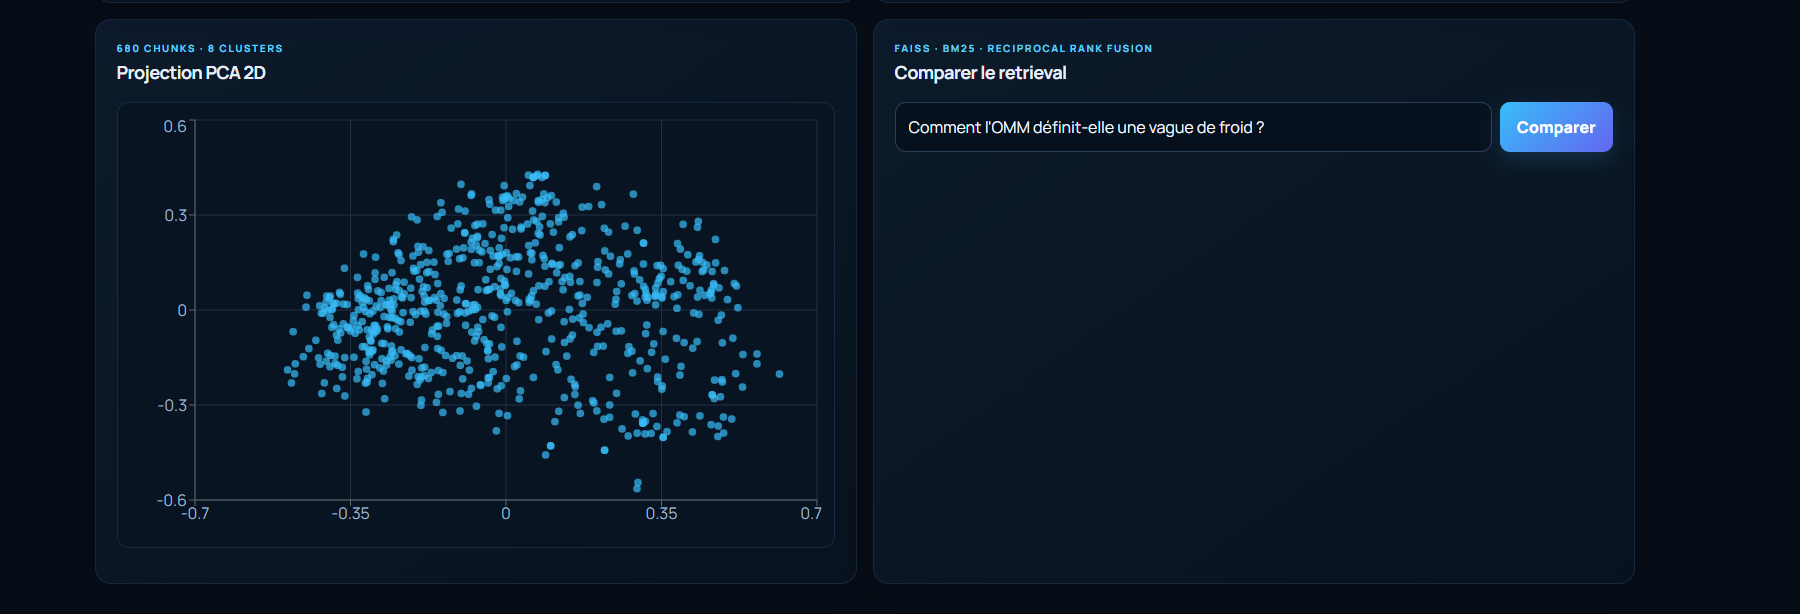
\includegraphics[width=0.95\linewidth]{interface_pca_retrieval.png}
\caption{Projection PCA 2D et comparaison FAISS / BM25 / RRF}
\end{figure}
\end{landscape}

\section{Résultats du Knowledge Graph}
Le graphe calculé contient 66 nœuds et 171 relations. La densité est de 0,078788 et la modularité Louvain de 0,281170. Seize communautés sont détectées. Certaines petites communautés correspondent à des entités faiblement reliées, tandis que le noyau central regroupe les concepts les plus fréquemment associés.

\begin{table}[H]
\centering
\caption{Métriques structurelles du Knowledge Graph}
\begin{tabular}{lr}
\toprule
\textbf{Métrique} & \textbf{Valeur}\\
\midrule
Nombre de nœuds & 66\\
Nombre de relations & 171\\
Densité & 0,078788\\
Communautés Louvain & 16\\
Modularité & 0,281170\\
Types de relations & 5 principaux\\
\bottomrule
\end{tabular}
\end{table}

\begin{figure}[H]
\centering
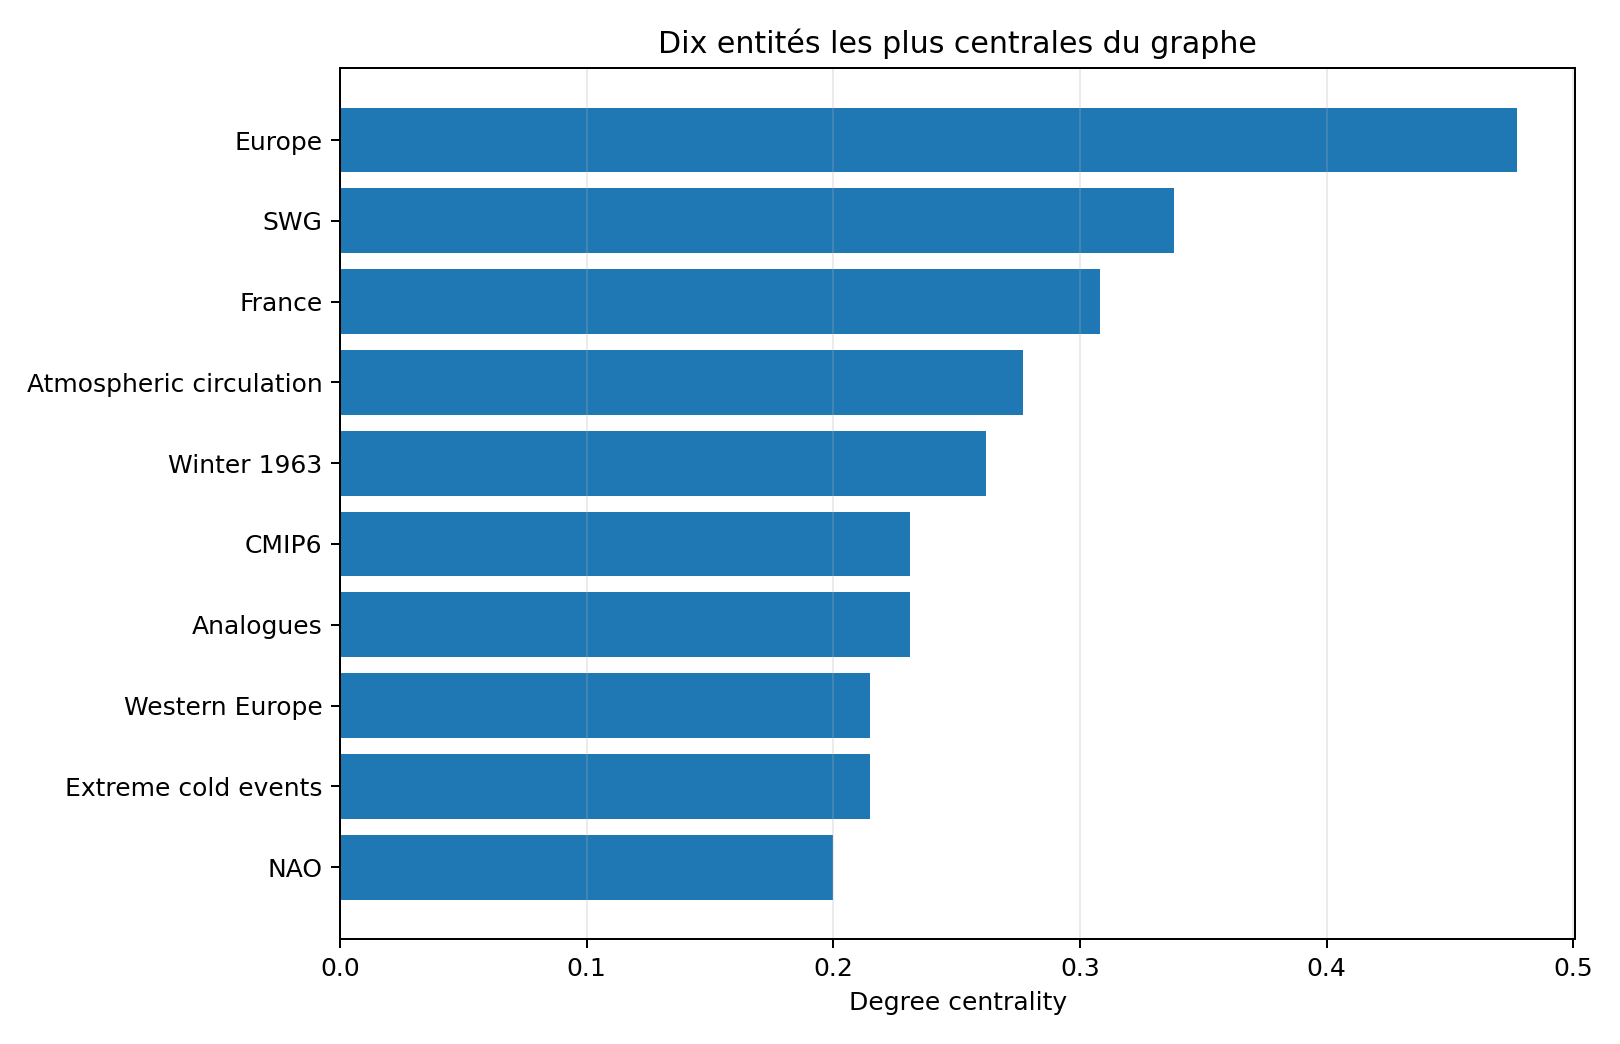
\includegraphics[width=0.92\textwidth]{chart_centrality.png}
\caption{Entités les plus centrales selon la degree centrality}
\end{figure}

\begin{table}[H]
\centering
\caption{Dix nœuds centraux du graphe}
\begin{tabular}{lr}
\toprule
\textbf{Entité} & \textbf{Degree centrality}\\
\midrule
Europe & 0,477\\
SWG & 0,338\\
France & 0,308\\
Atmospheric circulation & 0,277\\
Winter 1963 & 0,262\\
CMIP6 & 0,231\\
Analogues & 0,231\\
Western Europe & 0,215\\
Extreme cold events & 0,215\\
NAO & 0,200\\
\bottomrule
\end{tabular}
\end{table}

\begin{landscape}
\begin{figure}[H]
\centering
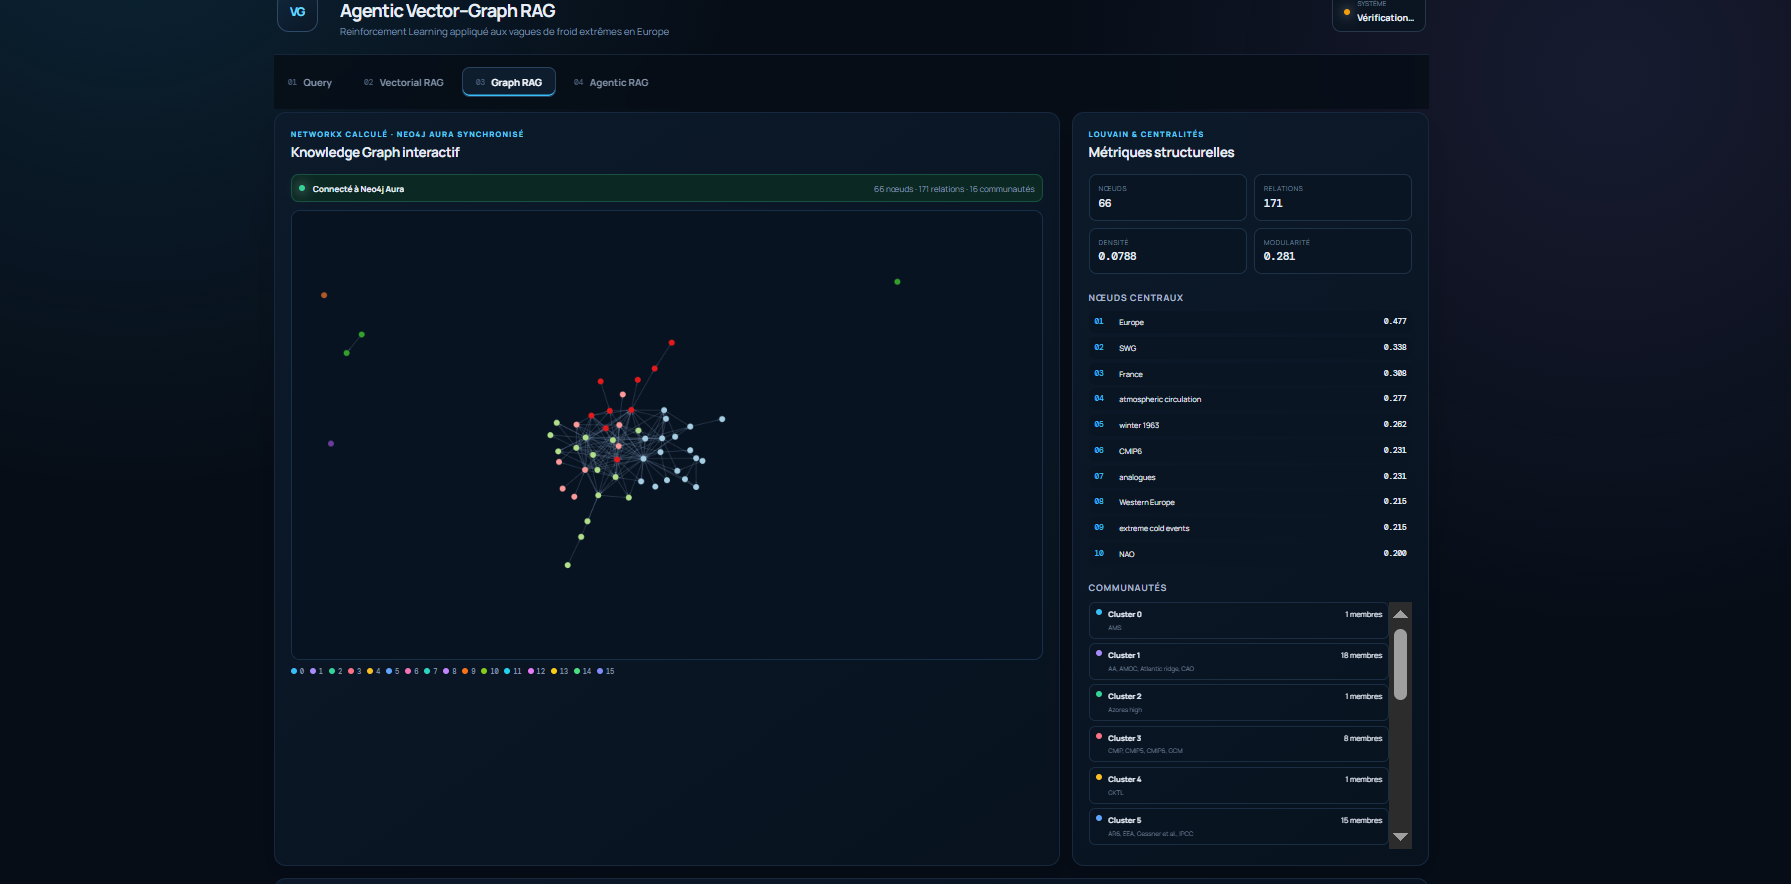
\includegraphics[width=0.92\linewidth]{interface_graph.png}
\caption{Onglet Graph RAG : communautés, centralités et statut Aura}
\end{figure}
\end{landscape}

\subsection{Vérification dans Neo4j Aura}
Deux synchronisations idempotentes donnent les mêmes totaux. La console Aura affiche les nœuds \tech{Entity}, les relations et les propriétés. Une relation sélectionnée expose son \tech{chunk\_id}, son score de confiance et l'extrait source.

\begin{figure}[H]
\centering
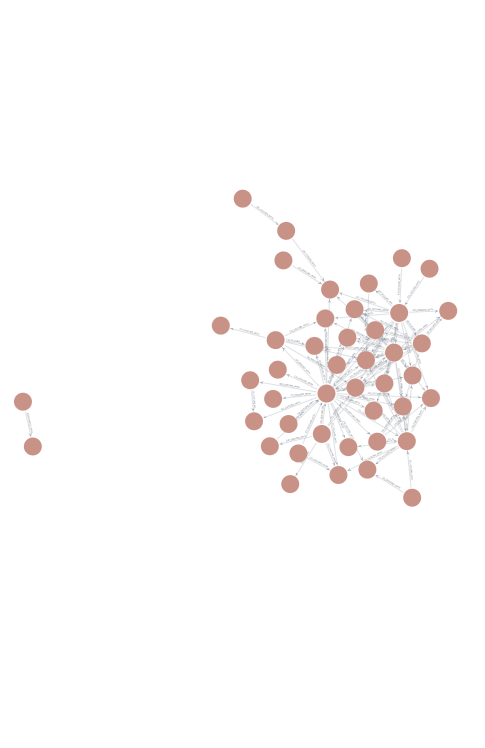
\includegraphics[height=0.52\textheight]{aura_graph.png}
\caption{Visualisation du graphe dans Neo4j Aura}
\end{figure}

\begin{landscape}
\begin{figure}[H]
\centering
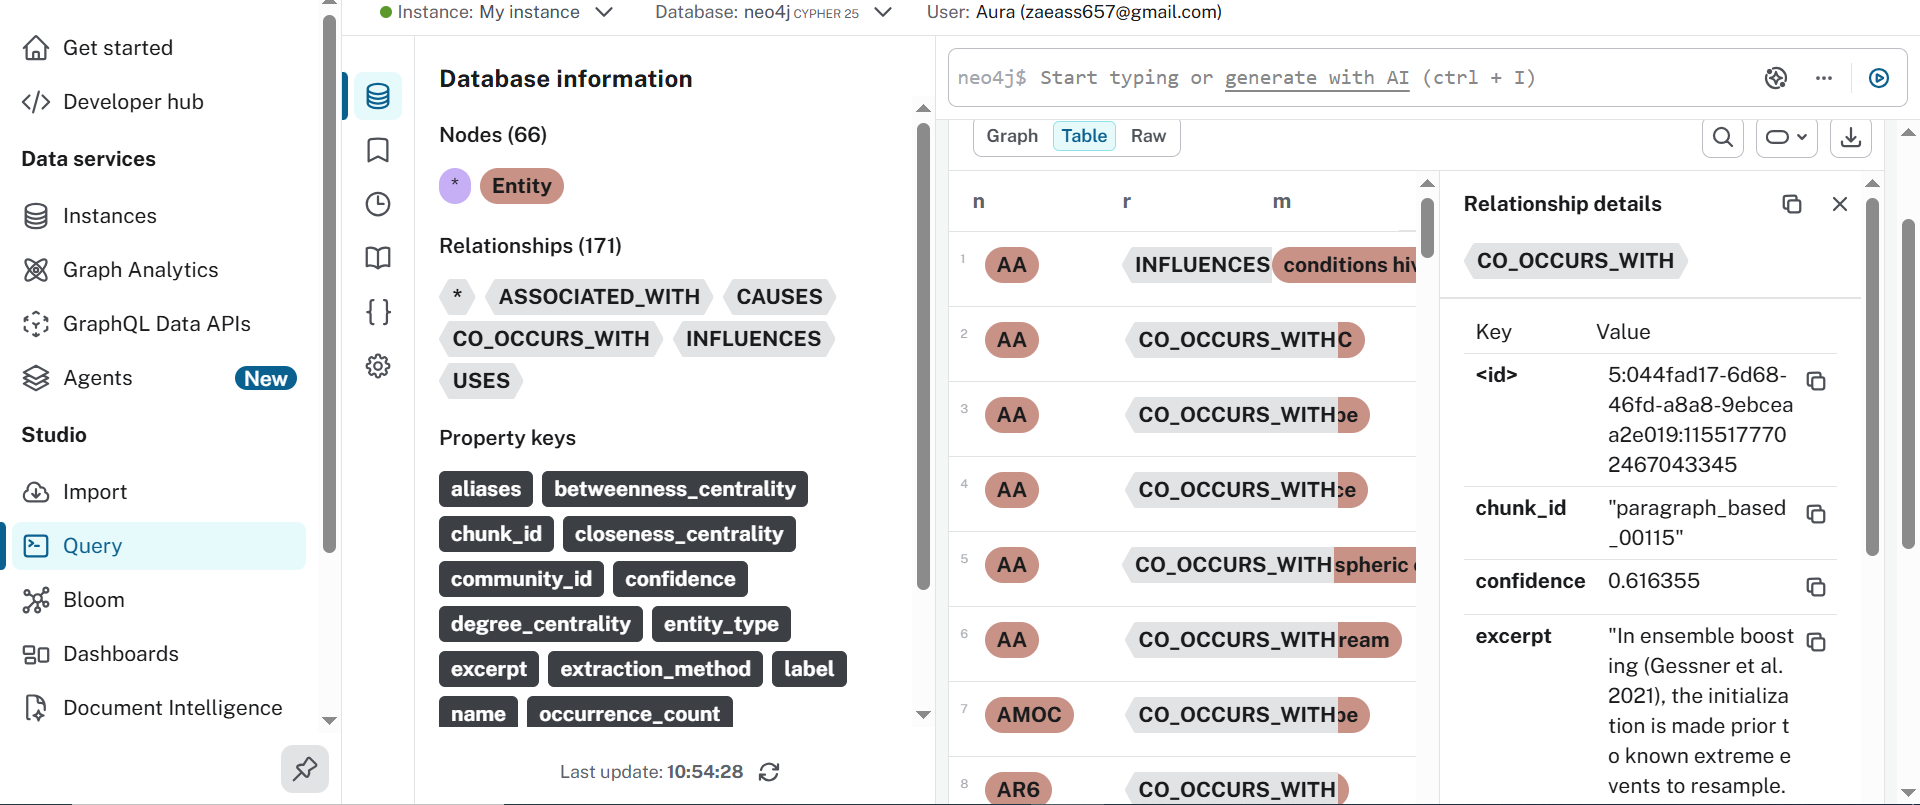
\includegraphics[width=0.95\linewidth]{aura_console_cropped.png}
\caption{Console Aura : 66 nœuds, 171 relations et détails de provenance}
\end{figure}
\end{landscape}

Les types de relations visibles sont \tech{ASSOCIATED\_WITH}, \tech{CAUSES}, \tech{CO\_OCCURS\_WITH}, \tech{INFLUENCES} et \tech{USES}. Les propriétés des nœuds comprennent les alias, le type d'entité, le nombre d'occurrences, la communauté et trois centralités.

\section{Résultats du Q-Learning et de LangGraph}
Le système utilise 16 états et quatre actions. L'entraînement fait décroître epsilon de 0,30 à 0,05. La Q-table finale associe les états sémantiques à \tech{use\_vector}, les états relationnels à \tech{use\_graph}, les états hybrides à \tech{use\_hybrid} et les états inconnus à \tech{abstain}.

Sur les huit questions de test annotées, le routage atteint 100\% et l'abstention correcte 100\%. Ce résultat doit être interprété dans le périmètre du petit jeu de test ; il ne constitue pas une garantie universelle sur toute formulation possible.

\begin{table}[H]
\centering
\caption{Exemples représentatifs de la politique apprise}
\begin{tabularx}{\textwidth}{Xrrrrl}
\toprule
\textbf{État} & \textbf{Vector} & \textbf{Graph} & \textbf{Hybrid} & \textbf{Abstain} & \textbf{Action}\\
\midrule
semantic$|$entity=0$|$coverage=high & 2,350 & -0,234 & -0,315 & -0,252 & use\_vector\\
relational$|$entity=1$|$coverage=high & -0,194 & 2,350 & -0,497 & -0,242 & use\_graph\\
hybrid$|$entity=1$|$coverage=high & -0,308 & -0,400 & 2,050 & -0,484 & use\_hybrid\\
unknown$|$entity=0$|$coverage=low & négatif & négatif & négatif & maximum & abstain\\
\bottomrule
\end{tabularx}
\end{table}

\begin{landscape}
\begin{figure}[H]
\centering
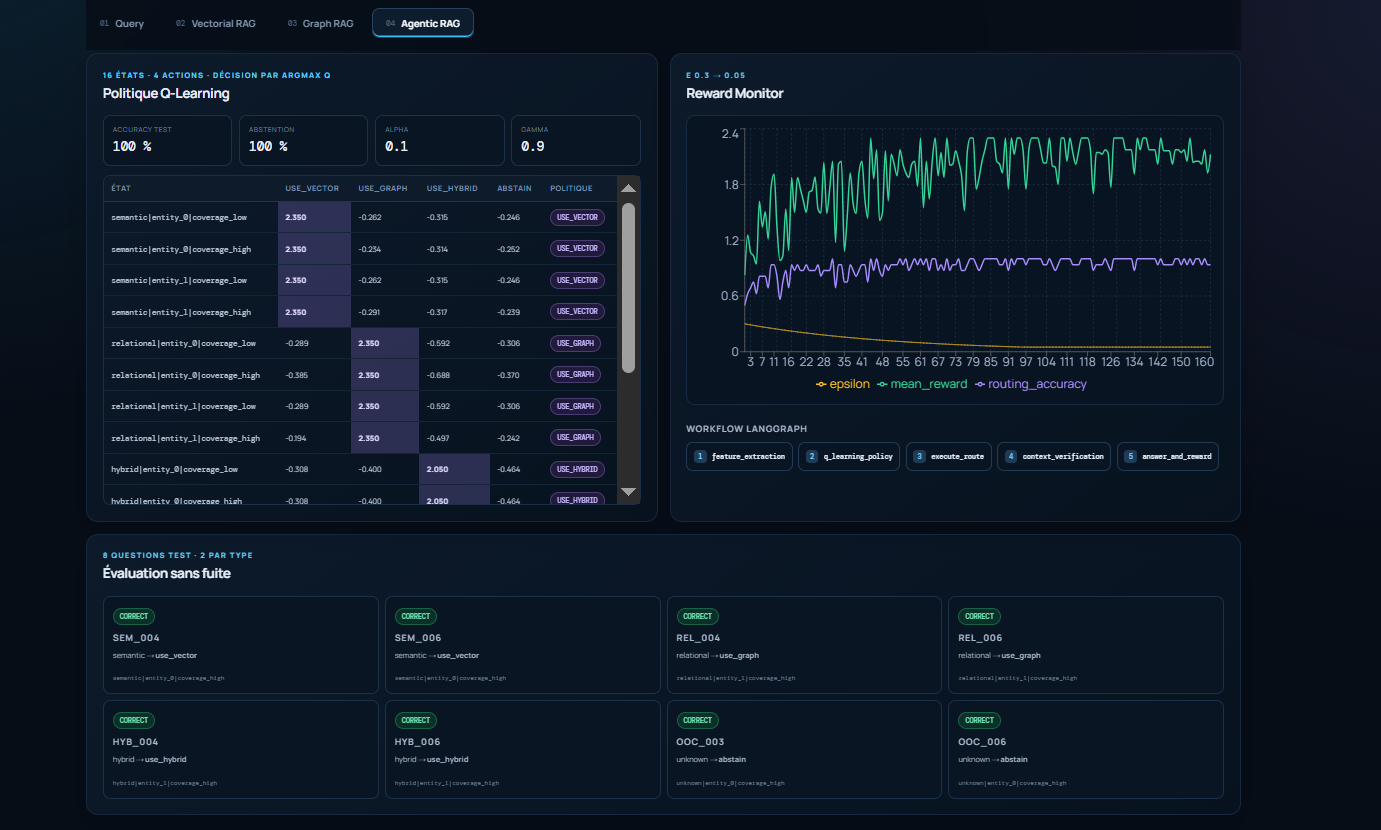
\includegraphics[width=0.94\linewidth]{interface_agentic.png}
\caption{Onglet Agentic RAG : Q-table, reward monitor et tests}
\end{figure}
\end{landscape}

La courbe de reward augmente puis se stabilise, tandis que l'epsilon diminue. La routing accuracy converge vers une valeur élevée. Le workflow LangGraph affiche explicitement les cinq nœuds exécutés, ce qui confirme que l'orchestration n'est pas remplacée par un appel direct.

\section{Backend FastAPI et frontend React}
Le backend charge les artefacts au démarrage et expose des réponses JSON. Le frontend interroge les endpoints avec des appels asynchrones et rend les tableaux, barres, scatter plots, graphes et cartes de provenance.

\begin{table}[H]
\centering
\small
\caption{Endpoints principaux de l'API}
\begin{tabularx}{\textwidth}{p{0.12\textwidth}p{0.31\textwidth}X}
\toprule
\textbf{Méthode} & \textbf{Route} & \textbf{Rôle}\\
\midrule
POST & /query & Pipeline agentique complet\\
GET & /vectorial & Résumé Vector RAG\\
GET & /vectorial/chunking & Métriques des sept chunkings\\
GET & /vectorial/embeddings & Métriques des représentations\\
POST & /vectorial/retrieve & FAISS, BM25 et RRF\\
GET & /graph & Nœuds, arêtes et statistiques\\
GET & /graph/communities & Louvain et membres\\
POST & /graph/subgraph & Cypher et sous-graphe\\
GET & /agentic & Q-table et rewards\\
GET & /query/history & Historique de session\\
\bottomrule
\end{tabularx}
\end{table}

\begin{landscape}
\begin{figure}[H]
\centering
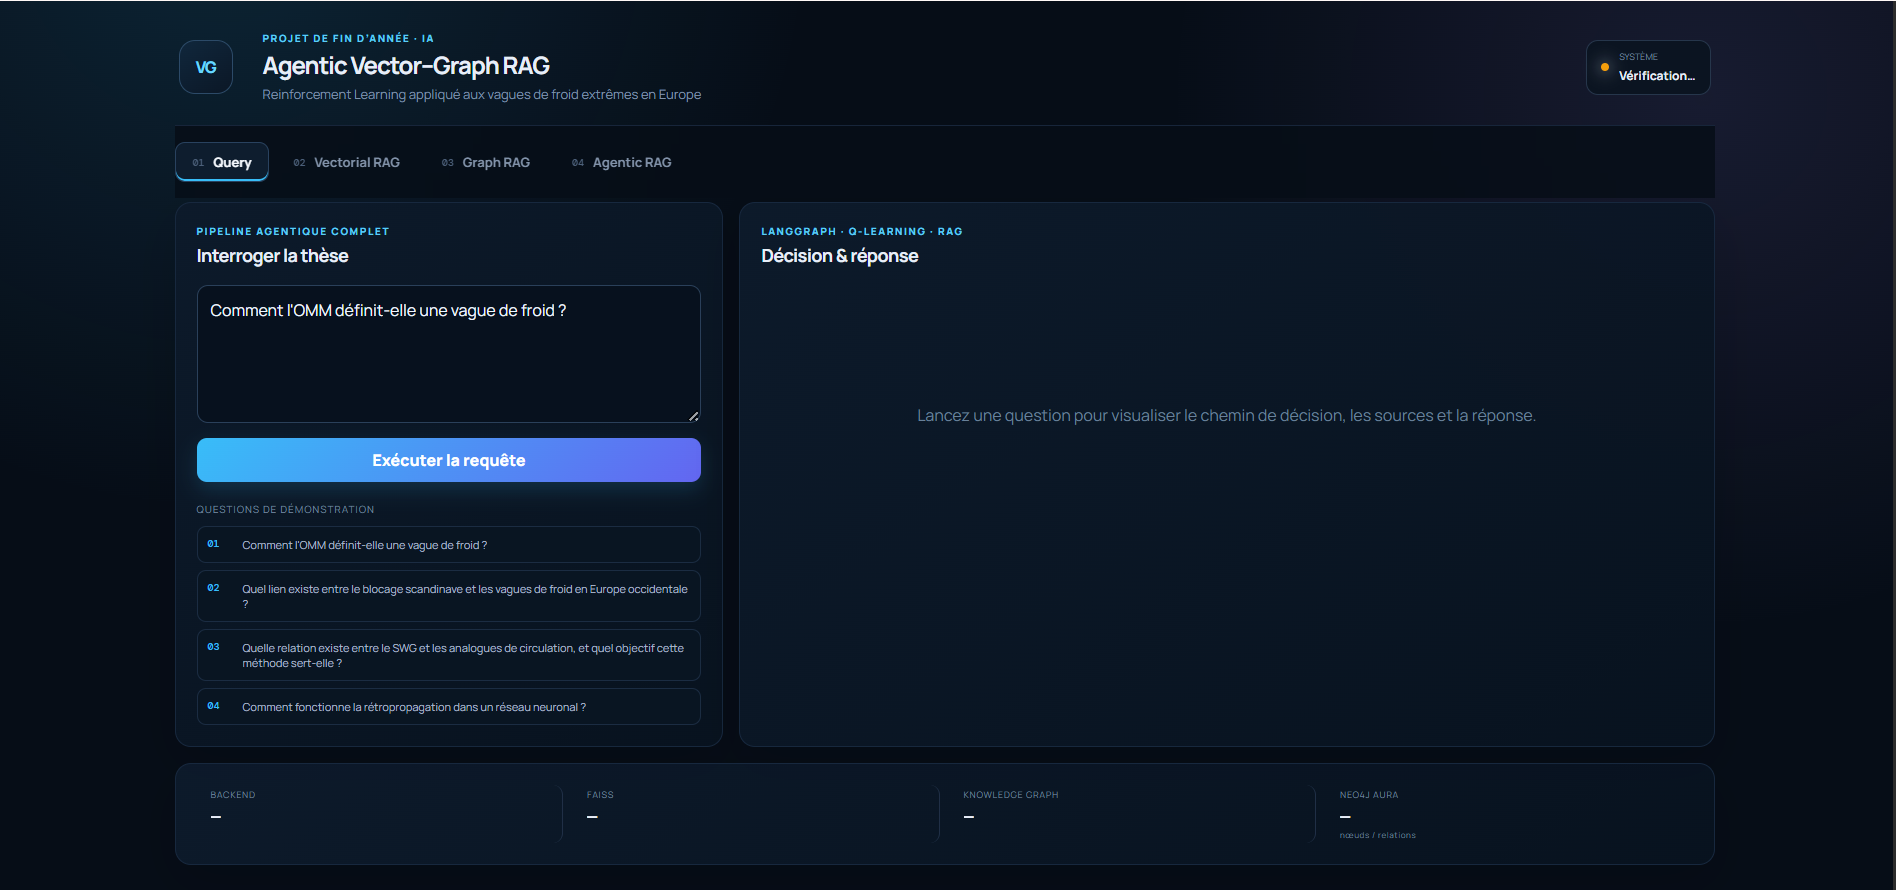
\includegraphics[width=0.95\linewidth]{interface_query.png}
\caption{Onglet Query avant exécution d'une question}
\end{figure}
\end{landscape}


\section{Analyse d'erreurs et étude d'ablation}
\subsection{Erreurs observées pendant l'ingestion}
Les erreurs les plus critiques ne provenaient pas des modèles, mais de la préparation du texte. Une césure mal recollée modifie un token, un ordre de colonnes incorrect détruit une phrase et un titre isolé peut être classé parmi les top chunks. Cette observation justifie la place importante accordée aux tests d'ingestion.

Un exemple visible dans la requête OMM est le chunk \tech{paragraph\_based\_00045}, qui contient principalement un titre de section. Il apparaît en troisième position avec un score inférieur aux deux passages de définition. Ce résultat n'est pas bloquant, mais il suggère une amélioration future : filtrer les chunks composés uniquement d'un titre ou leur appliquer un poids réduit.

\subsection{Ablation du modèle multilingue}
Lorsque les représentations lexicales remplacent MiniLM, le système retrouve plus difficilement les passages anglais à partir de questions françaises. TF-IDF caractères améliore partiellement les acronymes et les formes proches, mais son NDCG@5 reste à 0,289 contre 0,500 pour MiniLM.

\subsection{Ablation du graphe}
Sans Graph RAG, une question relationnelle peut encore retrouver un passage par FAISS, mais l'interface ne peut pas présenter le chemin entre les entités ni la requête Cypher. La réponse perd alors une partie de son explicabilité structurelle.

\subsection{Ablation de l'abstention}
Sans l'action \tech{abstain}, l'agent serait obligé de sélectionner un retriever, même pour la rétropropagation ou la grippe. Un passage faiblement similaire pourrait être transformé en réponse trompeuse. L'abstention est donc une fonction de sûreté, pas une absence de performance.

\section{Mesures de performance et comportement en démonstration}
Le coût principal de MiniLM est l'encodage initial de 680 chunks, mesuré à environ 24,2 secondes. Une fois l'index sauvegardé, une requête ne réencode que la question. Le graphe et la Q-table sont également chargés depuis le disque. Cette architecture garantit un démarrage prévisible et des réponses interactives.

Le script de lancement ouvre deux services locaux : le frontend sur le port 5173 et l'API sur le port 8000. La documentation Swagger est disponible sur le port 8000 avec le chemin \tech{/docs}. Le statut système vérifie le backend, FAISS, le graphe local et Aura.

\begin{table}[H]
\centering
\caption{Comportement attendu des composants pendant la démonstration}
\begin{tabularx}{\textwidth}{p{0.25\textwidth}p{0.25\textwidth}X}
\toprule
\textbf{Composant} & \textbf{Phase coûteuse} & \textbf{Comportement en ligne}\\
\midrule
Ingestion & Lecture des 206 pages & Aucun re-parsing\\
Chunking & Sept segmentations & Méthode gagnante chargée\\
Embeddings & Encodage des chunks & Encodage de la requête uniquement\\
FAISS / BM25 & Construction des index & Top-k immédiat\\
Graphe & Extraction et Louvain & Requête de sous-graphe\\
Q-Learning & Entraînement sur 16 questions & Argmax dans la Q-table\\
\bottomrule
\end{tabularx}
\end{table}

\section{Lecture détaillée des quatre onglets}
L'onglet Query constitue la démonstration du pipeline complet. L'onglet Vectorial RAG expose les choix expérimentaux et montre que le système n'a pas sélectionné arbitrairement une méthode. L'onglet Graph RAG prouve la persistance et l'analyse structurelle. L'onglet Agentic RAG explique le routage et l'apprentissage.

L'ordre des onglets traduit donc une progression : question utilisateur, preuves vectorielles, structure relationnelle puis décision agentique. Pendant la soutenance, cette progression évite de présenter immédiatement la Q-table sans avoir expliqué les outils qu'elle sélectionne.

\section{Scénarios fonctionnels de validation}
\subsection{Scénario sémantique : définition de l'OMM}
La question « Comment l'OMM définit-elle une vague de froid ? » est classée \tech{semantic}. L'état est \tech{semantic|entity\_0|coverage\_high} et l'action sélectionnée est \tech{use\_vector}. Le système retourne une confiance de 73\% et un contexte de 65\%.

Les chunks \tech{paragraph\_based\_00047}, \tech{00046} et \tech{00045} sont affichés avec les scores 0,646, 0,641 et 0,583. La page PDF 19 contient la définition de la WMO. Le résultat démontre la recherche cross-lingue et la conservation de la provenance.

\subsection{Scénario hybride : SWG et analogues}
La question « Qu'est-ce qu'un Stochastic Weather Generator et pourquoi est-il utilisé dans cette thèse ? » est classée hybride, car elle demande une explication textuelle et une relation avec l'objectif du travail. L'action est \tech{use\_hybrid}, la confiance 90\% et le contexte 100\%.

FAISS retrouve des passages des pages PDF 7, 39 et 55. Neo4j reçoit une requête Cypher sur les entités \textit{SWG}, \textit{analogues of circulation} et \textit{extreme cold events}. La réponse explique que le SWG repose sur les analogues et sert à simuler des événements de froid extrême dans une approche de type storyline.

\subsection{Scénario relationnel : blocage scandinave}
La question relationnelle doit sélectionner \tech{use\_graph}. Le système identifie le blocage scandinave, l'Europe occidentale et les vagues de froid, puis récupère les relations et leurs extraits. Le sous-graphe permet de visualiser l'advection d'air froid et l'affaiblissement des vents d'ouest.

\subsection{Scénario hors contexte}
La question « Comment fonctionne la rétropropagation dans un réseau neuronal ? » ne concerne pas le corpus. L'état inconnu conduit à l'action \tech{abstain}, et le système retourne exactement « Je ne sais pas ». Ce test vérifie que le moteur n'utilise pas ses connaissances générales pour fabriquer une réponse.

\section{Protocole de test et qualité logicielle}
La suite finale comprend 114 tests réussis. Elle couvre l'environnement, l'ingestion, la pagination, les caractères Unicode, les césures, la reconstruction des paragraphes, les métriques, la mise à jour Q-Learning, le chargement des artefacts, les endpoints et les scénarios critiques.

Le frontend compile avec \tech{npm run build}. L'API répond sur le port 8000 et Swagger permet de tester les schémas. Le script de lancement a été vérifié après fermeture complète des services, ce qui évite de confondre une page déjà ouverte avec un démarrage réussi.

\begin{table}[H]
\centering
\caption{Checklist finale de démonstration}
\begin{tabularx}{0.94\textwidth}{p{0.08\textwidth}X}
\toprule
\textbf{État} & \textbf{Vérification}\\
\midrule
OK & Backend, frontend, FAISS et Aura chargés\\
OK & Sept chunkings et sept représentations affichés\\
OK & PCA et comparaison des retrievers visibles\\
OK & 66 nœuds, 171 relations, 16 communautés\\
OK & Q-table, rewards et policy visibles\\
OK & Quatre routes de questions validées\\
OK & Réponse hors contexte : « Je ne sais pas »\\
OK & 114 tests et build React réussis\\
\bottomrule
\end{tabularx}
\end{table}

\section{Limites et perspectives techniques}
Le jeu d'évaluation reste limité. Une extension future devrait ajouter davantage de questions, plusieurs annotateurs et une mesure d'accord. Le graphe pourrait être enrichi avec des relations temporelles et des références bibliographiques, tout en conservant un seuil de confiance.

La synthèse extractive réduit l'hallucination mais peut produire un style moins naturel. Un petit LLM local pourrait être ajouté après validation, avec une contrainte stricte au contexte. Un reranker cross-encoder améliorerait potentiellement le top-k, mais augmenterait la latence. Enfin, un explorateur de chunks interactif permettrait de cliquer sur les points de la PCA et d'ouvrir le texte complet.

\section{Conclusion du chapitre}
Les résultats confirment que le MVP répond aux exigences obligatoires. Les comparaisons ne sont pas simulées, le graphe est réellement présent dans Aura, la Q-table pilote le routage et l'interface expose les preuves. La principale prudence concerne la taille du jeu de test ; les pourcentages de routage doivent toujours être présentés avec ce contexte.

% =============================================================================
% CONCLUSION
% =============================================================================
\chapter*{Conclusion Générale et Perspectives}
\addcontentsline{toc}{chapter}{Conclusion Générale et Perspectives}
Ce Projet de Fin d'Année a permis de construire un assistant documentaire complet à partir d'une thèse scientifique de 206 pages. Le travail ne s'est pas limité à intégrer une bibliothèque RAG. Il a exigé une chaîne expérimentale reproductible : nettoyage du corpus, comparaison des segmentations, comparaison des représentations, sélection mesurée, création d'un index vectoriel, construction d'un Knowledge Graph et apprentissage d'une politique de routage.

La méthode paragraph-based a obtenu le meilleur score global parmi sept chunkings, avec 680 chunks. Le modèle multilingue MiniLM a dominé les six autres représentations sur MAP, MRR et NDCG@5. Ces choix répondent au caractère cross-lingue du corpus. Le Vector RAG permet de retrouver des définitions et des explications, tandis que le Graph RAG représente les relations entre 66 entités à travers 171 arêtes et 16 communautés.

Le Q-Learning constitue la couche de décision. Il choisit parmi Vector, Graph, Hybrid et Abstain à partir de la Q-table. LangGraph orchestre les étapes et l'interface expose le chemin de décision. Le système ne dépend pas d'une API de LLM génératif ; la réponse extractive s'appuie uniquement sur les passages récupérés, avec des pages et des scores.

La démonstration finale permet de montrer non seulement que le système répond, mais aussi comment il répond. Une question sémantique affiche ses chunks, une question relationnelle affiche son Cypher et son sous-graphe, une question hybride combine les deux sources et une question hors sujet conduit à « Je ne sais pas ». La console Aura confirme la persistance réelle du Knowledge Graph et de sa provenance.

Les perspectives prioritaires sont l'élargissement du jeu d'évaluation, l'ajout d'un reranker léger, l'amélioration de l'explorateur de chunks et l'expérimentation d'un LLM local contraint. Le prototype peut également être généralisé à d'autres corpus, à condition de reconstruire l'ontologie, le jeu d'évaluation et les seuils de confiance. La contribution principale du projet reste une architecture transparente et mesurable, dans laquelle la qualité du retrieval et la provenance priment sur une génération non vérifiable.

\clearpage
\chapter*{Bibliographie et Webographie}
\addcontentsline{toc}{chapter}{Bibliographie et Webographie}
\begin{thebibliography}{99}
\bibitem{cadiou2025} C. Cadiou, \textit{Une approche statistique pour l'étude de l'intensité et de la dynamique des vagues de froid extrêmes en Europe}, Thèse de doctorat, Université Paris-Saclay, 2025.
\bibitem{lewis2020} P. Lewis et al., ``Retrieval-Augmented Generation for Knowledge-Intensive NLP Tasks'', NeurIPS, 2020.
\bibitem{johnson2019} J. Johnson, M. Douze et H. Jégou, ``Billion-scale similarity search with GPUs'', IEEE Transactions on Big Data, 2019.
\bibitem{robertson2009} S. Robertson et H. Zaragoza, ``The Probabilistic Relevance Framework: BM25 and Beyond'', Foundations and Trends in Information Retrieval, 2009.
\bibitem{reimers2019} N. Reimers et I. Gurevych, ``Sentence-BERT: Sentence Embeddings using Siamese BERT-Networks'', EMNLP-IJCNLP, 2019.
\bibitem{watkins1992} C. Watkins et P. Dayan, ``Q-learning'', Machine Learning, vol. 8, 1992.
\bibitem{sutton2018} R. Sutton et A. Barto, \textit{Reinforcement Learning: An Introduction}, MIT Press, 2018.
\bibitem{blondel2008} V. Blondel et al., ``Fast unfolding of communities in large networks'', Journal of Statistical Mechanics, 2008.
\bibitem{hagberg2008} A. Hagberg, D. Schult et P. Swart, ``Exploring network structure, dynamics, and function using NetworkX'', SciPy, 2008.
\bibitem{jolliffe2002} I. Jolliffe, \textit{Principal Component Analysis}, Springer, 2002.
\bibitem{neo4j} Neo4j, \textit{Neo4j and Cypher Documentation}, documentation technique consultée pour le stockage du graphe.
\bibitem{langgraph} LangChain, \textit{LangGraph Documentation}, documentation technique de l'orchestration par graphes d'états.
\bibitem{fastapi} S. Ramírez, \textit{FastAPI Documentation}, documentation de l'API Python.
\bibitem{react} Meta Open Source, \textit{React Documentation}, documentation de la couche de présentation.
\bibitem{wmo} World Meteorological Organization, lignes directrices et définition des événements de froid citées dans le corpus source.
\end{thebibliography}

% =============================================================================
% ANNEXES
% =============================================================================
\begin{appendices}
\chapter{Annexes Techniques : Pipeline et Configuration}

\section{Arborescence logique du projet}
\begin{lstlisting}[style=code]
pfa-agentic-graph-rag/
|-- backend/
|   |-- app/
|   |   |-- main.py
|   |   `-- core/mvp/
|   |-- data/
|   |   |-- processed/
|   |   |-- artifacts/
|   |   `-- metrics/
|   |-- eval/eval_set.json
|   |-- scripts/
|   |   |-- fast_build_mvp.py
|   |   `-- push_to_neo4j.py
|   `-- tests/test_mvp.py
|-- frontend/src/App.jsx
|-- run_mvp.bat
`-- rebuild_artifacts.bat
\end{lstlisting}

\section{Configuration Neo4j}
Les secrets ne sont jamais inclus dans le code ni dans le rapport. Le fichier local \tech{backend/.env}, ignoré par Git, suit le schéma suivant :
\begin{lstlisting}[style=code]
NEO4J_URI=neo4j+s://<instance>.databases.neo4j.io
NEO4J_USER=neo4j
NEO4J_PASSWORD=<secret-local>
NEO4J_DATABASE=neo4j
\end{lstlisting}

La vérification de connectivité exécute \tech{driver.verify\_connectivity()} puis la requête \tech{RETURN 1 AS connection\_test}. La synchronisation emploie \tech{MERGE} pour éviter les doublons.

\section{Extrait simplifié du workflow de requête}
\begin{lstlisting}[style=code,language=Python]
def query_pipeline(question: str) -> dict:
    features = extract_features(question)
    state = build_discrete_state(features)
    action = q_policy.select_action(state, exploration=False)

    if action == "use_vector":
        context = vector_retriever.retrieve(question, top_k=5)
    elif action == "use_graph":
        context = graph_retriever.retrieve(question)
    elif action == "use_hybrid":
        context = merge_contexts(
            vector_retriever.retrieve(question, top_k=5),
            graph_retriever.retrieve(question),
        )
    else:
        return {"answer": "Je ne sais pas.", "route": "abstain"}

    if not context_is_sufficient(context):
        return {"answer": "Je ne sais pas.", "route": action}

    return build_extractive_answer(context, state, action)
\end{lstlisting}

\section{Extrait de requête Cypher}
\begin{lstlisting}[style=code]
MATCH (n:Entity)-[r]-(m:Entity)
WHERE size($names) = 0
   OR n.name IN $names
   OR m.name IN $names
WITH n, r, m
ORDER BY coalesce(n.degree_centrality, 0.0) DESC
LIMIT 60
RETURN properties(n) AS source,
       type(r) AS relation_type,
       properties(r) AS relation,
       properties(m) AS target
\end{lstlisting}

\chapter{Annexes Techniques : Jeu d'Évaluation}
\section{Répartition des questions}
Le jeu contient 24 questions françaises : 6 sémantiques, 6 relationnelles, 6 hybrides et 6 hors contexte. Il est divisé en 16 questions d'entraînement et 8 questions de test. Les niveaux de difficulté sont équilibrés : 8 faciles, 8 moyens et 8 difficiles.

\section{Questions de démonstration}
\begin{enumerate}
  \item Comment l'OMM définit-elle une vague de froid ?
  \item Quel lien existe entre le blocage scandinave et les vagues de froid en Europe occidentale ?
  \item Quelle relation existe entre le SWG et les analogues de circulation, et quel objectif cette méthode sert-elle ?
  \item Comment fonctionne la rétropropagation dans un réseau neuronal ?
\end{enumerate}

Les sorties attendues sont respectivement \tech{use\_vector}, \tech{use\_graph}, \tech{use\_hybrid} et \tech{abstain}. La quatrième question doit retourner exactement « Je ne sais pas ».

\section{Autres exemples de questions}
\begin{longtable}{p{0.13\textwidth}p{0.68\textwidth}p{0.15\textwidth}}
\toprule
\textbf{Type} & \textbf{Question} & \textbf{Route}\\
\midrule
\endfirsthead
\toprule
\textbf{Type} & \textbf{Question} & \textbf{Route}\\
\midrule
\endhead
Semantic & Quelle différence la thèse établit-elle entre une cold wave et un cold spell ? & Vector\\
Semantic & Pourquoi un modèle multilingue est-il nécessaire pour interroger ce corpus ? & Vector\\
Relational & Quelle phase de la NAO est associée à l'hiver 1963 ? & Graph\\
Relational & Quels concepts sont directement reliés à CMIP6 dans le graphe ? & Graph\\
Hybrid & Comment le courant-jet relie-t-il la NAO négative aux vagues de froid ? & Hybrid\\
Hybrid & Quels passages et quelles relations décrivent l'utilisation du SWG ? & Hybrid\\
OOC & Quels sont les symptômes de la grippe saisonnière ? & Abstain\\
OOC & Comment configurer un routeur Wi-Fi ? & Abstain\\
\bottomrule
\end{longtable}

\chapter{Annexes Techniques : Routes API et Artefacts}
\section{Catalogue détaillé des routes}
\begin{longtable}{p{0.12\textwidth}p{0.33\textwidth}p{0.48\textwidth}}
\toprule
\textbf{Méthode} & \textbf{Route} & \textbf{Description}\\
\midrule
\endfirsthead
\toprule
\textbf{Méthode} & \textbf{Route} & \textbf{Description}\\
\midrule
\endhead
POST & /query & Route complète, confiance, décision, chunks, pages, Cypher et réponse\\
GET & /vectorial & Résumé de la méthode de chunking et de la représentation retenues\\
GET & /vectorial/chunking & Tableau des sept méthodes et métriques\\
GET & /vectorial/chunking/preview & Aperçu des chunks d'une méthode\\
GET & /vectorial/embeddings & Résultats des sept représentations\\
GET & /vectorial/pca & Coordonnées PCA et clusters\\
POST & /vectorial/retrieve & Comparaison des retrievers\\
GET & /graph & Nœuds, relations et statistiques\\
GET & /graph/communities & Communautés Louvain et modularité\\
GET & /graph/metrics & Densité et centralités\\
POST & /graph/subgraph & Sous-graphe d'une question et Cypher\\
GET & /graph/neo4j/status & État de la connexion Aura\\
GET & /agentic & Q-table, politique et rewards\\
POST & /agentic/train & Relance contrôlée de l'entraînement\\
POST & /agentic/feedback & Mise à jour par feedback\\
POST & /agentic/reset & Réinitialisation de la Q-table\\
GET & /query/history & Historique de la session\\
\bottomrule
\end{longtable}

\section{Artefacts produits}
\begin{table}[H]
\centering
\caption{Principaux artefacts persistants}
\begin{tabularx}{\textwidth}{p{0.43\textwidth}X}
\toprule
\textbf{Fichier} & \textbf{Contenu}\\
\midrule
metrics\_chunking.json & Statistiques et score global des chunkings\\
metrics\_embeddings.json & Métriques IR des représentations\\
graph.json & Nœuds et relations du Knowledge Graph\\
graph\_metrics.json & Densité, modularité, centralités et communautés\\
q\_table.json & Valeurs apprises pour les 16 états\\
reward\_history.json & Évolution du reward et de l'epsilon\\
neo4j\_sync\_report.json & Vérification de connexion et totaux Aura\\
faiss.index & Index vectoriel persistant\\
\bottomrule
\end{tabularx}
\end{table}


\chapter{Annexes Techniques : Algorithmes et Schémas de Données}
\section{Pseudo-code de comparaison des chunkings}
\begin{lstlisting}[style=code,language=Python]
for method in chunking_methods:
    chunks = method.split(corpus_pages)
    index = reference_embedder.encode(chunks)
    metrics = evaluate_retrieval(
        questions=evaluation_set,
        chunks=chunks,
        embeddings=index,
        ground_truth="page_level",
        k=5,
    )
    metrics.update(descriptive_statistics(chunks))
    save_json(method.name, metrics)

winner = max(all_metrics, key=global_chunking_score)
\end{lstlisting}

Le même modèle de référence est utilisé pour tous les chunkings. Cette contrainte évite qu'une méthode bénéficie d'un meilleur embedding et permet d'attribuer la différence aux frontières de segmentation.

\section{Pseudo-code de mise à jour Q-Learning}
\begin{lstlisting}[style=code,language=Python]
def q_update(state, action, reward, next_state):
    current = q_table[state][action]
    target = reward + gamma * max(q_table[next_state].values())
    q_table[state][action] = current + alpha * (target - current)
\end{lstlisting}

L'agent n'est pas entraîné sur les questions de test. Les huit questions de test servent uniquement à mesurer la politique finale. Les seeds fixes permettent de reconstruire les mêmes courbes et les mêmes Q-values.

\section{Schéma JSON d'un chunk}
\begin{lstlisting}[style=code]
{
  "chunk_id": "paragraph_based_00046",
  "method": "paragraph_based",
  "text": "The World Meteorological Organisation defines...",
  "page_pdf": 19,
  "page_these": 4,
  "chapter": "Introduction",
  "section": "Definition of extreme cold events",
  "language": "en",
  "word_count": 92
}
\end{lstlisting}

\section{Schéma JSON d'une relation}
\begin{lstlisting}[style=code]
{
  "source": "SWG",
  "relation_type": "USES",
  "target": "analogues of circulation",
  "chunk_id": "paragraph_based_00173",
  "confidence": 0.88,
  "excerpt": "Stochastic Weather Generator based on analogues...",
  "page_pdf": 39,
  "community_id": 5
}
\end{lstlisting}

\section{Structure d'une réponse API}
\begin{lstlisting}[style=code]
{
  "query_type": "hybrid",
  "action": "use_hybrid",
  "route": "Hybrid Vector-Graph RAG",
  "confidence": 0.90,
  "context_score": 1.00,
  "answer": "Le générateur stochastique de temps...",
  "decision_path": [
    "feature_extraction",
    "q_learning_policy",
    "execute_route",
    "context_verification",
    "extractive_answer"
  ],
  "chunks": [],
  "entities": [],
  "cypher": "MATCH ...",
  "subgraph": {}
}
\end{lstlisting}

\chapter{Annexes : Guide de Démonstration}
\section{Ordre recommandé pour la soutenance}
\begin{enumerate}
  \item Lancer \tech{run\_mvp.bat} et vérifier les quatre statuts.
  \item Ouvrir Vectorial RAG, montrer les sept chunkings et le gagnant.
  \item Montrer les sept représentations et expliquer le choix multilingue.
  \item Présenter la PCA et comparer FAISS, BM25 et RRF.
  \item Ouvrir Graph RAG, montrer 66 nœuds, 171 relations et 16 communautés.
  \item Exécuter une question dans Aura et afficher le sous-graphe.
  \item Ouvrir Agentic RAG, expliquer les états, actions, Q-values et rewards.
  \item Exécuter les quatre questions de démonstration.
  \item Terminer par la réponse « Je ne sais pas » pour montrer l'abstention.
\end{enumerate}

\section{Points à expliquer oralement}
Le chunking et les embeddings sont comparés hors ligne, une seule fois lors de la construction. À chaque question, le système n'essaie pas de nouveau les sept méthodes. Il utilise directement paragraph-based et MiniLM, déjà sélectionnés.

Le Q-Learning ne choisit pas la méthode de chunking. Il choisit seulement la route Vector, Graph, Hybrid ou Abstain. Les features construisent l'état, puis la Q-table fournit l'action de plus grande valeur.

MiniLM est un modèle d'intelligence artificielle local, mais pas un LLM génératif. Il produit des embeddings. La réponse finale est extractive, ce qui explique l'absence de clé API OpenAI, Claude ou Gemini.

\section{Commandes de vérification Aura}
\begin{lstlisting}[style=code]
MATCH (n) RETURN count(n) AS nodes;
MATCH ()-[r]->() RETURN count(r) AS relationships;
MATCH (n)
RETURN n.community_id AS community, count(n) AS members
ORDER BY members DESC;
MATCH (n)-[r]->(m) RETURN n, r, m LIMIT 100;
\end{lstlisting}

\end{appendices}

\end{document}
